% Create a one-sided article document type
\documentclass[a4paper, twoside, 12pt]{article}

% Define the course variables that are gonna be used several times
\newcommand{\university}{Universidad\ Politécnica\ de\ Madrid}
\newcommand{\school}{Escuela\ Técnica\ Superior\ de\ Ingenieros Informáticos}
\newcommand{\degree}{Grado\ Universitario\ en\ Ingeniería Informática}    
\newcommand{\tfg}{Trabajo de Fin de Grado}
\newcommand{\name}{XXXXX}
\newcommand{\me}{Pablo Palomo López}
\newcommand{\supervisor}{Óscar Corcho García}

% Configure the metadata of the PDF document
\usepackage[
	bookmarks       = true,             % Show the bookmarks
	unicode         = true,             % Use Unicode                 
	pdftoolbar      = true,             % Show Acrobat’s toolbar
	pdfmenubar      = true,             % Show Acrobat’s menu
	pdffitwindow    = false,            % Window fit to page when opened
	pdfstartview    = {FitH},           % Fit the page width to the window
	pdfauthor       = {\me},            % The author of this document
	pdftitle        = {\name\ --\ \me}, % The title of this document
	pdfsubject      = {\name},          % The subject of this document
	pdfkeywords     = {\name},          % The keywords of this document
	pdfnewwindow    = true,             % Open the links in a new PDF window
	colorlinks      = true,             % Use colored links
	linkcolor       = blue,             % Internal links color
	citecolor       = green,            % Bibliographic links color
	filecolor       = cyan,             % File links color
	urlcolor        = magenta           % External links color
]{hyperref}
\pdfstringdefDisableCommands{\let\uppercase}

% Redefine the size and margins (delete the 'twoside' indentation)
\usepackage[a4paper]{geometry}
% Define the geometry of the document
\newgeometry {
    top = 2.2cm, 
    bottom = 2.2cm, 
    right = 2cm, 
    left = 2cm
}
% Use UTF-8 as input encoding
\usepackage[utf8]{inputenc}
% Use a modern font (that is not pixelated)
\usepackage{lmodern}
% Use microtype to improve readability
\usepackage[protrusion = true, expansion = true]{microtype} 
% Use multiple columns
\usepackage{multicol}
% Display two figures next to each other
\usepackage{subfigure}
\usepackage[subfigure]{tocloft}
% Display list of Equations
\usepackage{tocloft}
% Insert empty pages
\usepackage{afterpage}

% Custom packages
% Font specification
\usepackage{fontspec}
\setmainfont[
    ItalicFont=NewCM10-Italic.otf,
    BoldFont=NewCM10-Bold.otf,
    BoldItalicFont=NewCM10-BoldItalic.otf,
    SmallCapsFeatures={Numbers=OldStyle}]
{NewCM10-Regular.otf}
\setsansfont[
    ItalicFont=NewCMSans10-Oblique.otf,
    BoldFont=NewCMSans10-Bold.otf,
    BoldItalicFont=NewCMSans10-BoldOblique.otf,
    SmallCapsFeatures={Numbers=OldStyle}]
{NewCMSans10-Regular.otf}
\setmonofont[
    Path=./fonts/,
    Extension=.ttf,
    BoldFont=*-SemiBold, % Semibold font as bold
    UprightFont=*-Regular, % Regular font as default
    ItalicFont=*-Medium, % Medium font as italic
    Scale=0.8]
{FiraCode}

% Graphic package for bullet points
\usepackage{graphicx}

% Hyperlinks
\usepackage{hyperref}
\hypersetup{
    colorlinks=true,
    linkcolor=blue,
    filecolor=magenta,      
    urlcolor=blue,
}
\urlstyle{same}

% Language highlighting
\usepackage{listings}
\lstdefinelanguage{lXML}{
    alsoletter={-},
    basicstyle=\ttfamily,
    breaklines=true,
    breakatwhitespace=true,
    frame=single,
    gobble=20,
    keywordstyle=[1]{\bfseries\color{RoyalBlue}},
    keywordstyle=[2]{\itshape\color{PineGreen}},
    keywordstyle=[3]{\color{RedViolet}},
    keywords=[1]{cac, cbc, cac-place-ext, cbc-place-ext},
    morekeywords=[2]{
        AddressLine,
        Attachment,
        AuctionConstraintIndicator,
        AuctionTerms,
        AwardDate,
        AwardedTenderedProject,
        BudgetAmount,
        CityName,
        Contact,
        Country,
        Description,
        ElectronicMail,
        EstimatedOverallContractAmount,
        ExternalReference,
        ContractFolderID,
        ContractFolderStatus,
        ContractFolderStatusCode,
        ContractingSystemCode,
        DurationMeasure,
        EndDate,
        ID,
        IdentificationCode,
        ItemClassificationCode,
        Language,
        LegalDocumentReference,
        LegalMonetaryTotal,
        Line,
        LocatedContractingParty,
        Name,
        Party,
        PartyName,
        PartyIdentification,
        PayableAmount,
        PlannedPeriod,
        PostalAddress,
        PostalZone,
        ProcedureCode,
        ProcurementProject,
        ProcurementProjectLot,
        ProcurementProjectLotID,
        ReceivedTenderQuantity,
        RequiredCommodityClassification,
        ResultCode,
        StartDate,
        SubmissionMethodCode,
        Telefax,
        Telephone,
        TenderingProcess,
        TenderingTerms,
        TenderResult,
        TotalAmount,
        TypeCode,
        URI,
        WebsiteURI,
        WinningParty
    },
    morekeywords=[3]{
        currencyID,
        languageID,
        listURI,
        schemeName,
        unitCode
    },
    morestring=*[d]{"},
    morestring=[s][]{\#\{}{\}},
    rulecolor=\color{black},
    showstringspaces=false,
    stringstyle=\color{OrangeRed}, 
    tabsize=10
}
\lstdefinelanguage{lJSON}{
    alsoletter={\{,\},\[,\]},
    basicstyle=\ttfamily,
    breaklines=true,
    breakatwhitespace=true,
    frame=single,
    gobble=20,
    keywordstyle=[1]{\bfseries},
    keywordstyle=[2]{\color{Brown}},
    keywordstyle=[3]{\color{Red}},
    keywords=[1]{\{,\},\[,\]},
    morekeywords=[2]{
        awards,
        parties,
        planning,
        tender
    },
    morekeywords=[3]{
        additionalIdentifiers,
        address,
        amount,
        budget,
        classification,
        contactPoint,
        countryName,
        currency,
        date,
        description_es,
        documents,
        documentType,
        email,
        endDate,
        faxNumber,
        id,
        identifier,
        items,
        locality,
        lots,
        mainProcurementCategory,
        name,
        ocid,
        postalCode,
        procurementMethod,
        procurementMethodDetails_es,
        relatedLot,
        roles,
        schema,
        startDate,
        streetAddress,
        submissionMethod,
        submissionMethodDetails,
        suppliers,
        tag,
        telephone,
        tenderPeriod,
        title,
        url,
        value
    },
    morestring=*[d]{"},
    morestring=[s][]{\#\{}{\}},
    rulecolor=\color{black},
    showstringspaces=false,
    stringstyle=\color{BrickRed},
    tabsize=10
}
% Fixed tabbing
\usepackage{tabto}

% Paragraph sections
\usepackage{titlesec}
\setcounter{secnumdepth}{4}

% Indexes name change
\renewcommand*\contentsname{Índice}
\renewcommand*\listtablename{Lista de tablas}

% Configure style aspects of the document
\usepackage{caption}            % To configure the captions
\usepackage{siunitx}            % For SI units
\usepackage{graphicx}           % To include graphics
\usepackage[dvipsnames]{xcolor} % To configure colors
\usepackage{fancyhdr}           % To configure the header and footer
\pagestyle{fancy}               % Use a fancy header style
\fancyhf{}                      % Set the header format
\fancyheadoffset{0.0 cm}        % Set the header offset
\lhead{\tfg}                    % Set the header right-side contents
\rhead{\name}                   % Set the header left-side contents
\cfoot{\thepage}                % Set the footer page number

% Table label change
\captionsetup[table]{name=Tabla}

% Create a custom command shortcut
\renewcommand{\arraystretch}{1.3} % Modify the vertical spacing of the tables
\raggedbottom                     % Modify the vertical spacing of enumerated environments

% Set empty page 
\newcommand\blankpage{%
    \null
    \thispagestyle{empty}%
    \addtocounter{page}{-1}%
    \newpage
}

% Set the title format
\title {
	\vspace*{1.0 cm}
	\Large\textbf{\uppercase{\university}} \\
	\vspace*{0.5 cm}
	\large\textbf{\uppercase{\school}} \\
	\vspace*{2 cm}
	\large\text{\uppercase{\degree}} \\
	\vspace*{2 cm}
	\large\text{\uppercase{\tfg}} \\
	\vspace*{1.0 cm}
	\LARGE\textbf{\uppercase{\name}} \\
}

% Set the author format
\author {
	\normalsize
	\begin{tabbing}
        \hspace*{0.4\linewidth} \= \hspace*{0.5\linewidth} \= \kill
    	\> Autor: \' \textbf{\me} \\[0.25cm]
    	\> Supervisor: \' \textbf{\supervisor} \\
    \end{tabbing}
    
    \vspace{2cm}
}

% Set the date format
\date { 
    Madrid, mayo de 2021
}

% A macro to print the title
\makeatletter
\def\printtitle{{\centering\@title\par}}
\makeatother

% A macro to print the author
\makeatletter
\def\printauthor{{\centering\large\@author}}
\makeatother

% A macro to print the date
\makeatletter
\def\printdate{{\centering\@date}}
\makeatother

%%%%%%%%%%%%%%%%%%%%%%%%%%%%%%%%%%%%%%%%%%%%%%%%%%%%%%%
% Start the document
\begin{document}
    % Include the cover
    \afterpage{\blankpage}
    \thispagestyle{empty} % Remove page numbering on this page

\begin{center}
    
    \centering
    \begin{figure}[h!]
        \centering
        \begin{subfigure}
            \centering
            % Include UPM's logo
        	
\includegraphics[width = 0.5\linewidth, height = 3cm, keepaspectratio]{images/UPM.eps}
    	\end{subfigure}
    	\hspace{3cm}%
    	\centering
        \begin{subfigure}
            \centering
            % Include ETSII's logo
        	
\includegraphics[width = 0.5\linewidth, height = 3cm, keepaspectratio]{images/ETSII.eps}
        \end{subfigure}
	\end{figure}
	
	% Print the title
	\printtitle
	
	% Add vertical padding
    \vfill
    
    % Print the author
    \printauthor
    
    % Print the date
    \printdate
\end{center}

\newpage              % Insert a page break
\setcounter{page}{1}  % Set the page counter
    % Include the different sections
    \addtocounter{page}{-1}

\vspace*{15em}
\section*{Abstract}
    \vspace{0.5cm}
    \begin{adjustwidth}{50pt}{50pt}
        \hspace{15pt} This paper explores both the current  publication state of the contracting data at national and European levels, as well as the methodologies of said publications: open and linked data. In addition, the two reference standards, \texttt{CODICE} and \texttt{OCDS}, are presented.
        \\ \\
        \indent Next, the developed software whose purpose is to execute the data transformation between the two standards, is presented. The implemented mappings are listed in the following section.
        \\ \\
        \indent Finally, the way system produced data is published as open linked data through the software deployment is described.
    \end{adjustwidth}
    \vspace{1cm}
    \hspace{0.5cm} \textbf{\textit{Keywords}}: public contracting, tender, open data, linked data, standard.

\phantomsection
\addcontentsline{toc}{section}{Abstract}

\newpage
    \vspace*{15em}

\begin{center}
    \section*{Resumen}
    
        ...

\end{center}

\phantomsection
\addcontentsline{toc}{section}{Resumen}

\newpage
    \vspace*{15em}

\begin{center}
    \section*{Acknowledgement}
    
        ...

\end{center}

\phantomsection
\addcontentsline{toc}{section}{Acknowledgement}

\newpage
    \tableofcontents

\newpage
    {%
    \let\oldnumberline\numberline%
    \renewcommand{\numberline}{Tabla~\oldnumberline}%
    \listoftables%
}
    {%
    \let\oldnumberline\numberline%
    \renewcommand{\numberline}{Figure~\oldnumberline}%
    \vspace{1cm}
    \listoffigures%
}

    \newcommand{\listequationsname}{\Large{List of Equations}}
\newlistof{myequations}{equ}{\listequationsname}
\newcommand{\myequations}[1]{
   \addcontentsline{equ}{myequations}{\protect\numberline{\theequation}#1}
}
\setlength{\cftmyequationsnumwidth}{3.75em}
\setlength{\cftmyequationsindent}{1.8em}

{%
    \let\oldnumberline\numberline%
    \renewcommand{\numberline}{Eq.~\oldnumberline}%
    \vspace{1cm}
    \listofmyequations%
}

\newpage
    \section{Introduction}

...

\newpage
    %\mysection{Software desarrollado} \label{sec:software}
    La presente sección describe el sistema software desarrollado, \textit{OCDS\_Mapper}, mediante el formato de un documento de diseño software (SDD, por sus siglas en inglés). En esta sección se proporcionar una visión general del sistema, desde su descripción hasta sus funcionalidades, de las que se derivan las características concretas que han sido implementadas.
    \\ \\
    La documentación del software que se describirá a continuación estará guiada por la norma \texttt{J-STD-016-1995} \cite{JSTD}, un estándar para el ciclo de vida de los procesos de desarrollo de software promulgado por dos de los organismos más relevantes en el área de las tecnologías de la información; la EIA (\textit{Electronic Industries Association}) y el IEEE (\textit{The Institute of Electrical and Electronics Engineers}).
    \\ \\
    En esta sección que especifica el diseño de la arquitectura del sistema previamente citado, se incluyen los siguientes apartados:
    \\
    \begin{itemize}
        \item Consideraciones de diseño
        \item Estructura de la aplicación
        \item Diseño de la arquitectura
        \item Diseño detallado del sistema
        \item Trazabilidad de requisitos
        \item Flujo de ejecución
        \item Cobertura de código
    \end{itemize}
    
    \subsection{Consideraciones de diseño}
        \subsubsection{Lenguaje de programación}
            La implementación del sistema se ha realizado mediante el \textit{framework} \texttt{.NET Core 5.0.202}, usando el lenguaje \texttt{C\#} bajo el estándar que describe su sintaxis e interpretación \cite{ISOCS}.
            
        \subsubsection{Arquitectura de componentes orientada a servicios}
            Con el objetivo de alcanzar la máxima abstracción de tareas posible, el sistema se ha diseñado de tal forma que cada componente realice un servicio concreto, con una funcionalidad bien definida, capaz de integrarse con el resto de componentes del sistema.
            \\ \\
            El \textit{OCDS\_Mapper}, por tanto, estará compuesto de componentes individuales, concretamente 4, descritos en la subsección \hyperref[subsubsec:componentes]{componentes software}.
            
        \subsubsection{Patrón de productor-consumidor}
            El sistema implementará el patrón de diseño software de productor-consumidor de la siguiente manera:
            \\ \\
            Las funcionalidades que implementen la recogida de datos, sea de manera local o remota, serán los productores, y las funcionalidades que implementen el procesado de los datos, esto es, el mapeado entre estándares, serán los consumidores.
            \\ \\
            Para asegurar un correcto flujo de recursos entre los componentes que sigan dichos roles se implementan mecanismos de sincronización y exclusión mutua entre ellos.
        
        \subsubsection{Mecanismo de consultas}
            Para realizar las búsquedas de elementos sobre los documentos de licitaciones de la Plataforma de Contratacíon Pública del Estado se ha utilizado la tecnología \textit{Language Integrated Query} (\texttt{LINQ}), propia del \textit{framework} \texttt{.NET}.
            \\ \\
            A través de \texttt{LINQ} se pueden realizar consultas sobre estructuras de datos mediante una sintaxis parecida a la del lenguaje \textit{Structured Query Language} (\texttt{SQL}). En concreto, para el tipo de datos que la aplicación obtiene (extensión \texttt{.atom}, formato \texttt{XML}), la rama de \texttt{LINQ} utilizada es \texttt{LINQ to XML} \cite{LINQXML}.
            \\ \\
            Para ejemplificar el funcionamiento de \texttt{LINQ}, se utilizará una sentencia utilizada en esta aplicación. Concretamente, el ejemplo provisto en la \hyperref[fig:linq]{figura 10} representa una consulta que busca el elemento raíz (\texttt{ContractFolderStatus}) de cada entrada de un documento de licitaciones.
            \\ \\
            \begin{lstlisting}[language=lCSharp,gobble=14]
                IEnumerable<XElement> query =
                    from node in entry.Elements()
                    where node.Name.LocalName.Equals("ContractFolderStatus")
                    select node;
            \end{lstlisting}
            \captionof{figure}{Ejemplo de una sentencia de \texttt{LINQ}}
            \label{fig:linq}
        
        \subsubsection{Librerías utilizadas} \label{subsubsec:libreria}
            El sistema utiliza distintas librerías para realizar la implementación de las funcionalidades requeridas. En concreto, estas librerías son:
            
            \begin{itemize}
                \item AsyncEx \cite{LIBASYNC}: Librería utilizada para el uso de colecciones aptas para la exclusión mutua. Licencia MIT \cite{LICMIT}.
                \item FluentAssertions \cite{LIBASSERT}: Librería de ayuda en la codificación de tests. Licencia Apache v2 \cite{LICAPACHE}.
                \item Microsoft.Extensions.Configuration \cite{LIBCONFIG}: Librería utilizada para pasar información a la aplicación mediante ficheros de configuración. Licencia MIT \cite{LICMIT}.
                \item NLog \cite{LIBNLOG}: Librería para llevar el registro del funcionamiento del sistema. Licencia BSD 3-Clause \cite{LICBSD3}.
                \item Json.NET \cite{LIBJSON}: Librería utilizada para la construcción de documentos en formato JSON. Licencia MIT \cite{LICMIT}.
                \item xUnit \cite{LIBXUNIT}: Librería para realizar el \textit{testing} del sistema. Liencia Apache v2 \cite{LICAPACHE}.
            \end{itemize}   
    
    \subsection{Estructura de la aplicación}
        La aplicación \textit{OCDS\_Mapper} (una \textit{solución}, en el ámbito de estructuras de proyectos en \textit{Visual Studio} \cite{VSPROJSOL}) está estructurada en dos \textit{proyectos}; \texttt{src} y \texttt{test}, con el código fuente del programa y el módulo de testeo de la aplicación, respectivamente. En la \hyperref[fig:estructura]{figura 11} se puede visualizar la estructura de directorios de la aplicación.
        \\ \\
        Además del fichero \texttt{Program.cs}, que incluye el punto de entrada de la aplicación, y el fichero de configuración \texttt{appsettings.json}, dentro del proyecto del código fuente de la aplicación se han estructurado los ficheros en los siguientes directorios:
        
        \begin{itemize}
            \item \texttt{Examples}: ejemplos de casos de uso de la aplicación.
                \begin{itemize}
                    \item \texttt{json}: ejemplos de documentos mapeados por la aplicación.
                    \item \texttt{xml}: ejemplos de documentos de la Plataforma de Contratación Pública.
                \end{itemize}
            \item \texttt{Exceptions}: excepciones propias del funcionamiento de la aplicación.
                \begin{itemize}
                    \item \texttt{EmptyMappingRuleException.cs}: se lanza si se provee una regla de mapeado vacía.
                    \item \texttt{InvalidOperationCodeException.cs}: se lanza si no se provee un modo de operación válido.
                    \item \texttt{InvalidParsedElementException.cs}: se lanza si no se encuentra el elemento raíz en una entrada de un documento de licitaciones.
                    \item \texttt{InvalidPathLengthException.cs}: se lanza si se provee una regla de mapeado de longitud inválida.
                    \item \texttt{WrongMappingException.cs}: se lanza si se encuentra un elemento inesperado en el mapeado de los datos.
                \end{itemize}
            \item \texttt{Interfaces}: interfaces de los componentes de la arquitectura.
                \begin{itemize}
                    \item \texttt{IMapper.cs}: interfaz del componente de mapeado de datos.
                    \item \texttt{IPackager.cs}: interfaz del componente de empaquetado de datos.
                    \item \texttt{IParser.cs}: interfaz del componente de parseo de datos.
                    \item \texttt{IProvider.cs}: interfaz del componente de provisión de datos.
                \end{itemize}
            \item \texttt{Model}: implementación de los componentes de la arquitectura.
                \begin{itemize}
                    \item \texttt{Mapper.cs}: implementación del componente de mapeado de datos.
                    \item \texttt{Packager.cs}: implementación del componente de empaquetado de datos.
                    \item \texttt{Parser.cs}: implementación del componente de parseo de datos.
                    \item \texttt{Provider.cs}: implementación del componente de provisión de datos.
                \end{itemize}
            \item \texttt{Utils}: ficheros con funcionalidades extra.
                \begin{itemize}
                    \item \texttt{Document.cs}: tipo de datos que abstrae una instancia de un documento de licitaciones.
                    \item \texttt{EnumCodes.cs}: fichero con los tipos enumerados del programa.
                    \item \texttt{Mappings.cs}: clase estática con las reglas de mapeado.
                \end{itemize}
        \end{itemize}
        
        En cuanto al proyecto de \textit{testing}, en los ficheros \texttt{UnitTests.cs} y \texttt{IntegrationTests.cs} se pueden encontrar las pruebas unitarias y de integración, respectivamente.
        
        \begin{figure}[h]
            \centering
            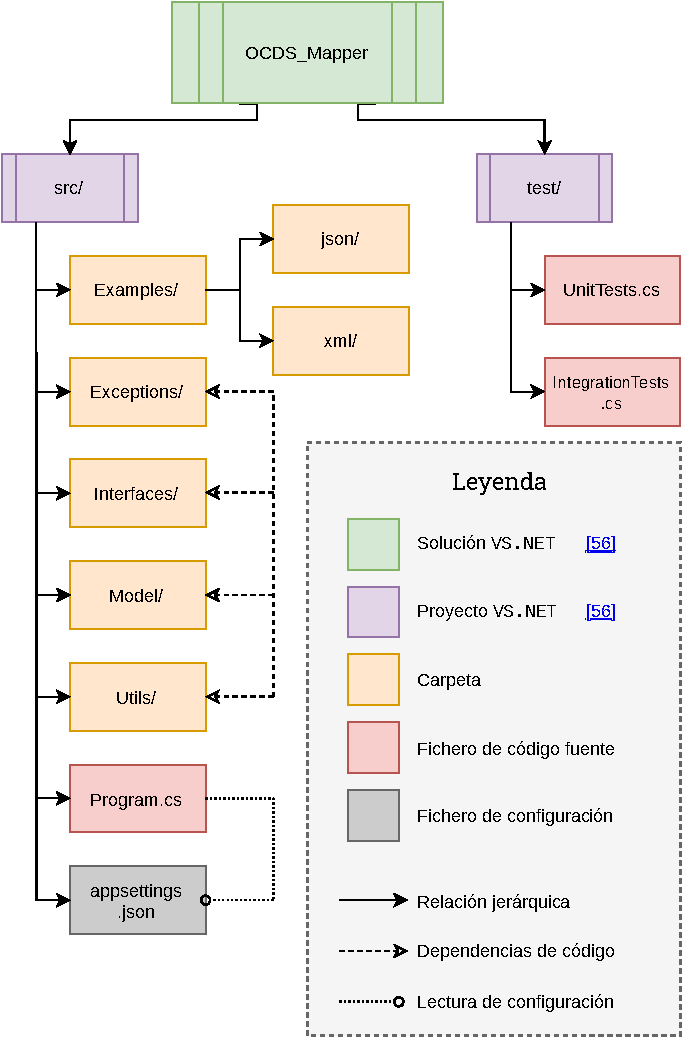
\includegraphics[width=0.65\textwidth]{estructura.pdf}
            \captionof{figure}{Diagrama de estructura de la aplicación}
            \label{fig:estructura}
        \end{figure}
        
    \subsection{Diseño de la arquitectura}
        \subsubsection{Componentes software} \label{subsubsec:componentes}
            Dado que el sistema está diseñado mediante una arquitectura de componentes orientada a servicios, el diseño de la arquitectura se limita a la propia descripción de los componentes que lo integran.
            \\ \\
            Posteriormente, en el \hyperref[subsec:detallado]{diseño detallado del sistema}, se incluirán los diagramas \texttt{UML} individuales de cada componente, acompañados en la sección de \hyperref[subsec:flujo]{flujo de ejecución} por una serie de diagramas de flujo con la representación de la ejecución del sistema.
            \\ \\
            Las interfaces de los componentes del sistema pueden encontrarse en el \hyperref[annex:interfaces]{Anexo I}.
            
            \begin{center}
                \begin{tabular}{|| M{3cm} | M{12cm} ||} 
                    \hline
                        Nombre del componente & Descripción del componente \\
                    \hline\hline
                        \textit{\large Provider} & Componente encargado de la provisión de los datos. Admite cuatro modos de operación: proveer el documento más reciente disponible, proveer un documento específico (ya sea local o en forma de \texttt{URL}), proveer los documentos correspondientes únicamente al día anterior, o proveer un flujo continuo de documentos desde el más reciente hasta no encontrar un fichero enlazado más o abortar la aplicación \\ 
                    \hline
                        \textit{\large Parser} & Componente encargado del parseo de los datos de los documentos de la Plataforma de Contratación Pública. Provee servicios para extraer los espacios de nombres, los elementos dadas sus rutas, etcétera  \\
                    \hline
                        \textit{\large Mapper} & Componente encargado del mapeado de los datos al estándar \texttt{OCDS}. A través de los elementos \texttt{XML} provistos por el \textit{Parser} y las reglas especificadas en \textit{Mappings}, construye el fichero \texttt{JSON} correspondiente al mapeado de cada entrada \texttt{XML} \\
                    \hline
                        \textit{\large Packager} & Componente encargado del empaquetado de los datos ya mapeados. Publica los paquetes de datos de manera local para su posterior carga y procesado a \texttt{RDF} \\
                    \hline
                \end{tabular}
            \end{center}
            \captionof{table}{Tabla de descripción de componentes}
            
            \vspace{0.3cm}
            
            \begin{figure}[h]
                \centering
                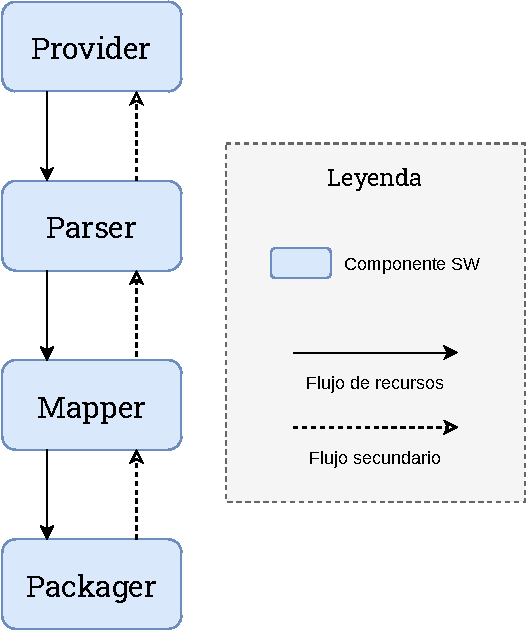
\includegraphics[width=0.5\textwidth]{componentes.pdf}
                \captionof{figure}{Diagrama de los componentes del sistema}
                \label{fig:componentes}
            \end{figure}
            
            En el diagrama de interrelación de componentes (véase \hyperref[fig:componentes]{figura 12}) se pueden apreciar dos tipos de flujo distintos.
\newpage
            El principal, el flujo de recursos, representa el funcionamiento básico del sistema: el componente de provisión de datos (\textit{Provider}) suministra los documentos con los datos de contrataciones públicas bajo el esquema \texttt{CODICE} al componente de extracción de datos (\textit{Parser}). Una vez los datos del documento han sido extraídos, por cada entrada del documento de contrataciones se genera una nueva instancia del componente de mapeado (\textit{Mapper}), que implementa las reglas de mapeado descritas en el componente estático \textit{Mappings}. Cuando el documento ha sido totalmente procesado, el componente de empaquetado de datos (\textit{Packager}) finaliza el pipeline del sistema, publicando los datos de manera local.
            \\ \\
            El flujo secundario representa el uso de métodos entre los distintos componentes, ya sea de manera estática o mediante llamadas a instancias de los componentes.
            
        \subsubsection{Especificación de requisitos}
            Este apartado recoge todos los requisitos, funcionales y de calidad del sistema, que han sido diseñados para la arquitectura del sistema.

            \begin{longtable}{|| M{3cm} | M{12cm} ||} 
                \hline
                    Código del requisito & Descripción del requisito \\
                \hline\hline
                    \texttt{\textit{RF-1}} & El sistema debe ser capaz de descargar documentos de la Plataforma de Contratación Pública \\ 
                \hline
                    \texttt{\textit{RF-2}} & El sistema debe ser capaz de recuperar el documento de licitaciones más reciente \\
                \hline
                    \texttt{\textit{RF-3}} & El sistema debe ser capaz de descargar un documento provisto con una ruta, sea de manera local o remota \\
                \hline
                    \texttt{\textit{RF-4}} & El sistema debe ser capaz de detectar que una ruta a un documento provisto, local o remota, sea incorrecta \\
                \hline
                    \texttt{\textit{RF-5}} & El sistema debe ser capaz de otorgar los documentos provistos de manera asíncrona y bloqueante \\
                \hline
                    \texttt{\textit{RF-6}} & El sistema debe ser capaz de eliminar aquellos documentos que ya hayan sido procesados \\
                \hline
                    \texttt{\textit{RF-7}} & El sistema debe ser capaz de recuperar los espacios de nombres del \texttt{XML} del documento de licitaciones \\
                \hline
                    \texttt{\textit{RF-8}} & El sistema debe ser capaz de proveer los documentos enlazados a los que se están procesando \\
                \hline
                    \texttt{\textit{RF-9}} & El sistema debe ser capaz de recopilar el conjunto de entradas que aparecen en cada documento de licitaciones \\
                \hline
                    \texttt{\textit{RF-10}} & El sistema debe ser capaz de establecer el elemento raíz de cada documento de licitaciones \\
                \hline
                    \texttt{\textit{RF-11}} & El sistema debe ser capaz de detectar que a un documento de licitaciones le falta el elemento raíz \\
                \hline
                    \texttt{\textit{RF-12}} & El sistema debe ser capaz de encontrar un elemento específico en el documento de licitaciones dada su ruta \\
                \hline
                    \texttt{\textit{RF-13}} & El sistema debe ser capaz de encontrar un conjunto de elementos específicos en el documento de licitaciones dada su ruta \\
                \hline
                    Código del requisito & Descripción del requisito \\
                \hline
                \hline
                    \texttt{\textit{RF-14}} & El sistema debe ser capaz de devolver el documento de licitaciones enlazado al que está siendo procesado actualmente \\
                \hline
                    \texttt{\textit{RF-15}} & El sistema debe ser capaz de encontrar un elemento específico a partir de otro en el documento de licitaciones \\
                \hline
                    \texttt{\textit{RF-16}} & El sistema debe ser capaz de devolver el valor de un código descrito en un documento de códigos \\
                \hline
                    \texttt{\textit{RF-17}} & El sistema debe ser capaz de construir un documento en formato \texttt{JSON} con el documento de licitaciones procesado \\
                \hline
                    \texttt{\textit{RF-18}} & El sistema debe ser capaz de detectar una regla de mapeado vacía \\
                \hline
                    \texttt{\textit{RF-19}} & El sistema debe ser capaz de detectar una regla de mapeado de longitud inválida \\
                \hline
                    \texttt{\textit{RF-20}} & El sistema debe ser capaz de detectar una regla de mapeado sin definir \\
                \hline
                    \texttt{\textit{RF-21}} & El sistema debe ser capaz de construir las colecciones de objetos \texttt{JSON} en el documento siendo mapeado \\
                \hline
                    \texttt{\textit{RF-22}} & El sistema debe ser capaz de mapear el elemento \texttt{ContractFolderStatusCode} en el elemento \texttt{tag} \\
                \hline
                    \texttt{\textit{RF-23}} & El sistema debe ser capaz de mapear el eleemnto \texttt{ContractFolderID} en el elemento \texttt{OCID} \\
                \hline
                    \texttt{\textit{RF-24}} & El sistema debe ser capaz de mapear el elemento \texttt{ProcurementProject/Name} en el elemento \texttt{tender.title} \\
                \hline
                    \texttt{\textit{RF-25}} & El sistema debe ser capaz de mapear el elemento \texttt{ProcurementProject/BudgetAmount/
                    EstimatedOverallContractAmount} en el elemento \texttt{tender.value} \\
                \hline
                    \texttt{\textit{RF-26}} & El sistema debe ser capaz de mapear el elemento \texttt{ProcurementProject/BudgetAmount/TotalAmount} en el elemento \texttt{budget.amount} \\
                \hline
                    \texttt{\textit{RF-27}} & El sistema debe ser capaz de mapear el elemento \texttt{ProcurementProject/PlannedPeriod/StartDate} en el elemento \texttt{tender.period.startDate} \\
                \hline
                    \texttt{\textit{RF-28}} & El sistema debe ser capaz de mapear el elemento \texttt{ProcurementProject/PlannedPeriod/EndDate} en el elemento \texttt{tender.period.endDate} \\
                \hline
                    \texttt{\textit{RF-29}} & El sistema debe ser capaz de mapear el elemento \texttt{ProcurementProject/PlannedPeriod/DurationMeasure} en el elemento \texttt{tender.period.durationInDays} \\
                \hline
                    \texttt{\textit{RF-30}} & El sistema debe ser capaz de mapear el elemento \texttt{ProcurementProject/TypeCode} en el elemento \texttt{tender.mainProcurementCategory} \\
                \hline
\newpage
                \hline
                    Código del requisito & Descripción del requisito \\
                \hline
                \hline
                    \texttt{\textit{RF-31}} & El sistema debe ser capaz de mapear el elemento \texttt{ProcurementProjectLot/ID} en los elementos \texttt{tender.lots.id, tender.items\{id, relatedLot\}} \\
                \hline
                    \texttt{\textit{RF-32}} & El sistema debe ser capaz de mapear el elemento \texttt{ProcurementProjectLot/ProcurementProject/BudgetAmount/
                    TotalAmount} en el elemento \texttt{tender.lots.value} \\
                \hline
                    \texttt{\textit{RF-33}} & El sistema debe ser capaz de mapear el elemento \texttt{ProcurementProjectLot/ProcurementProject/
                    RequiredCommodityClassification/ItemClassificationCode} en el elemento \texttt{tender.items.classification} \\
                \hline
                    \texttt{\textit{RF-34}} & El sistema debe ser capaz de mapear el elemento \texttt{TenderingProcess/ProcedureCode} en el elemento \texttt{tender.procurementMethod} \\
                \hline
                    \texttt{\textit{RF-35}} & El sistema debe ser capaz de mapear el elemento \texttt{TenderingProcess/ContractingSystemCode} en el elemento \texttt{tender.procurementMethodDetails\_es} \\
                \hline
                    \texttt{\textit{RF-36}} & El sistema debe ser capaz de mapear el elemento \texttt{TenderingProcess/SubmissionMethodCode} en el elemento \texttt{tender.submissionMethod} \\
                \hline
                    \texttt{\textit{RF-37}} & El sistema debe ser capaz de mapear el elemento \texttt{TenderingTerms/Language/ID} en el elemento \texttt{tender.submissionMethodDetails} \\
                \hline
                    \texttt{\textit{RF-38}} & El sistema debe ser capaz de mapear el elemento \texttt{TenderingProcess/AuctionTerms/AuctionConstraintIndicator} en el elemento \texttt{tender.submissionMethod} \\
                \hline
                    \texttt{\textit{RF-39}} & El sistema debe ser capaz de mapear el elemento \texttt{LocatedContractingParty/Party/PartyName/Name} en el elemento \texttt{parties[i].name} \\
                \hline
                    \texttt{\textit{RF-40}} & El sistema debe ser capaz de mapear el elemento \texttt{LocatedContractingParty/Party/PartyIdentification/ID} en los elementos \texttt{parties[i].\{additionalIdentifiers, id, identifier.\{id, schema\}, roles\}} \\
                \hline
                    \texttt{\textit{RF-41}} & El sistema debe ser capaz de mapear el elemento \texttt{LocatedContractingParty/Party/PostalAddress/Contact} en el elemento \texttt{parties[i].\{address, countryName, contactPoint\}} \\
                \hline
                    \texttt{\textit{RF-42}} & El sistema debe ser capaz de mapear el elemento \texttt{TenderResult/AwardedTenderedProject/ProcurementProjectID} en el elemento \texttt{awards[i].id} \\
                \hline
                    \texttt{\textit{RF-43}} & El sistema debe ser capaz de mapear el elemento \texttt{TenderResult/ResultCode} en el elemento \texttt{awards[i].status} \\
                \hline
\newpage
                \hline
                    Código del requisito & Descripción del requisito \\
                \hline
                \hline
                    \texttt{\textit{RF-44}} & El sistema debe ser capaz de mapear el elemento \texttt{TenderResult/WinningParty} en los elementos \texttt{\{awards[i].suppliers, parties[j]\}} \\
                \hline
                    \texttt{\textit{RF-45}} & El sistema debe ser capaz de mapear el elemento \texttt{TenderResult/AwardedTenderedProject/LegalMonetaryTotal/
                    PayableAmount} en el elemento \texttt{awards[i].value} \\
                \hline
                    \texttt{\textit{RF-46}} & El sistema debe ser capaz de mapear el elemento \texttt{TenderResult/ReceivedTenderQuantity} en el elemento \texttt{tender.numberOfTenderers} \\
                \hline
                    \texttt{\textit{RF-47}} & El sistema debe ser capaz de mapear el elemento \texttt{TenderResult/AwardDate} en el elemento \texttt{awards[i].date} \\
                \hline
                    \texttt{\textit{RF-48}} & El sistema debe ser capaz de mapear el elemento \texttt{TenderResult/Description} en el elemento \texttt{awards[i].description\_es} \\
                \hline
                    \texttt{\textit{RF-49}} & El sistema debe ser capaz de mapear el elemento \texttt{TenderResult/Contract/ID} en el elemento \texttt{contracts[i].id} \\
                \hline
                    \texttt{\textit{RF-50}} & El sistema debe ser capaz de mapear el elemento \texttt{TenderResult/StartDate} en el elemento \texttt{contracts[i].period.startDate} \\
                \hline
                    \texttt{\textit{RF-51}} & El sistema debe ser capaz de detectar las ocurrencias de los identificadores para prevenir los duplicados \\
                \hline
                    \texttt{\textit{RF-52}} & El sistema debe ser capaz de crear un paquete de entrega siguiendo el formato \texttt{OCDS} \\
                \hline
                    \texttt{\textit{RF-53}} & El sistema debe ser capaz de publicar un paquete de entrega de manera local \\
                \hline
                    \texttt{\textit{RF-54}} & El sistema debe ser capaz de detectar argumentos incorrectos \\
                \hline
                    \texttt{\textit{RF-55}} & El sistema debe ser capaz de detectar la falta de argumentos requeridos como el directorio de salida \\
                \hline
            \end{longtable}
            \addtocounter{table}{-1}
            \captionof{table}{Tabla de requisitos funcionales}
            

    
    \subsection{Diseño detallado del sistema} \label{subsec:detallado}
        \subsubsection{Casos de uso del componente de provisión de datos}
    
            \begin{figure}[h]
                \centering
                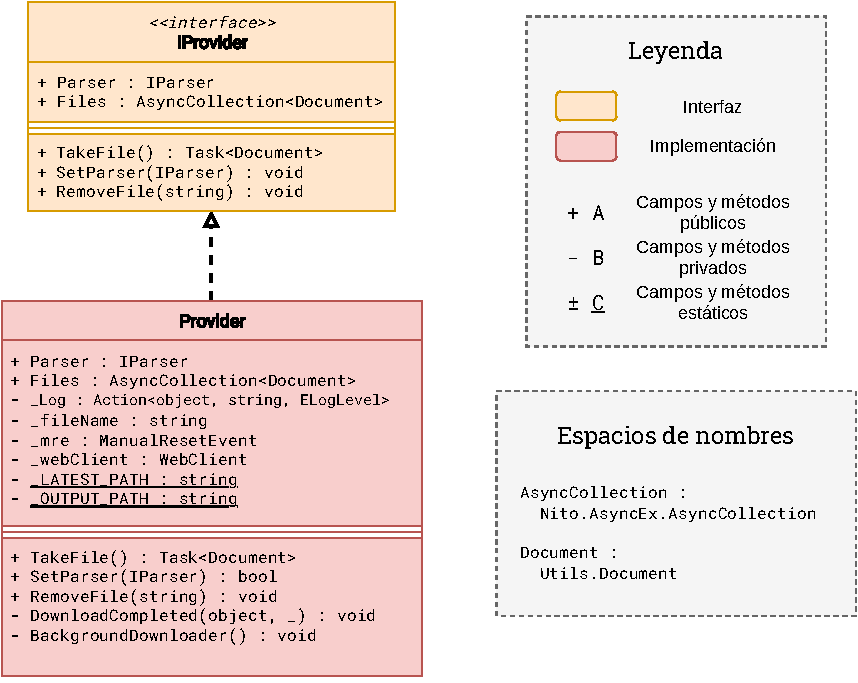
\includegraphics[width=0.8\linewidth]{provider.pdf}
                \captionof{figure}{Diagrama \texttt{UML} del componente \textit{Provider}}
                \label{fig:provider}
            \end{figure}
            
            \paragraph{Caso de uso I: modo de carga local} \mbox{}\\
                El componente de provisión de datos debe ser capaz de cargar en memoria para su posterior procesado un fichero localizado en el sistema de ficheros local de la máquina ejecutando el proceso. También debe notificar si la ruta al fichero local especificado no es correcta o si en ella no existe dicho fichero.
                
            \paragraph{Caso de uso II: modo de descarga remota} \mbox{}\\
                El componente de provisión de datos debe ser capaz de descargar para su posterior procesado un documento de licitaciones desde la Plataforma de Contratación Pública. También debe notificar si la \texttt{URL} no es correcta.
            
            \paragraph{Caso de uso III: provisión simple} \mbox{}\\
                El componente de provisión de datos debe ser, si así se especifica, capaz de proveer un único documento de licitaciones, el cual podrá ser cargado o descargado de manera local o remota, respectivamente. En el caso de una provisión simple de manera remota, el componente tratará de descargar aquel documento más reciente, cuya \texttt{URL} \cite{LICIDIA} queda descrita en el portal de datos abiertos del Ministerio de Hacienda \cite{PORTALHAC}.
                
            \paragraph{Caso de uso IV: provisión continua} \mbox{}\\
                El componente de provisión de datos debe ser capaz, si así se especifica, y sólo en el modo de descarga remota, de encontrar en el documento de licitaciones siendo descargado el enlace al siguiente documento, con el fin de proveer un flujo continuo de recursos para el procesado en el sistema. El primer documento del flujo será el más reciente, descrito en el apartado anterior.
                
            \paragraph{Caso de uso V: provisión diaria} \mbox{}\\
                El componente de provisión de datos debe ser capaz, si así se especifica, y sólo en el modo de descarga remota, de igual manera que con el caso de uso de la provisión continua, de proveer un flujo de recursos para ser procesados, con la salvedad que dicho flujo se limite exclusivamente al conjunto de documentos publicados en el día anterior.
                
        \subsubsection{Casos de uso del componente de parseo de datos}
    
            \begin{figure}[h]
                \centering
                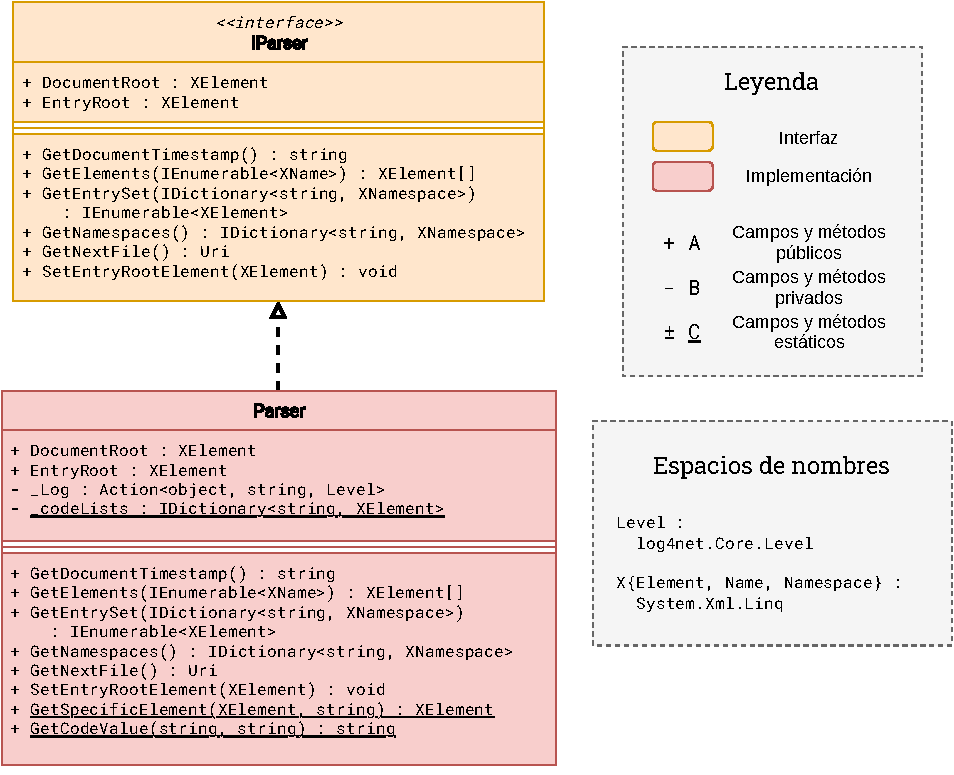
\includegraphics[]{parser.pdf}
                \captionof{figure}{Diagrama \texttt{UML} del componente \textit{Parser}}
                \label{fig:parser}
            \end{figure}
            
            \paragraph{Caso de uso I: extracción de elementos} \mbox{}\\
                El componente de parseo de datos debe ser capaz de extraer todos los elementos requeridos dado un documento de licitaciones. Los elementos de interés para ser extraídos son, entre otros, el \textit{timestamp} de la publicación, el conjunto de entradas, el conjunto de espacios de nombres, o la ruta al documento enlazado.
                
            \paragraph{Caso de uso II: extracción específica de elementos} \mbox{}\\
                El componente de parseo de datos debe ser capaz de, dada una ruta que iterar o un punto del que partir, bajar por los niveles del documento y extraer un elemento específico, con el objetivo de realizar posteriores mapeados lo más independientes posible.
            
            \paragraph{Caso de uso III: obtención de códigos} \mbox{}\\
                El componente de parseo de datos debe ser capaz de descargar en memoria aquellos documentos de códigos usados por el sistema y poder extraer de ellos los valores necesitados en cada momento.
\newpage
        \subsubsection{Casos de uso del componente de mapeado de datos}
    
            \begin{figure}[h]
                \centering
                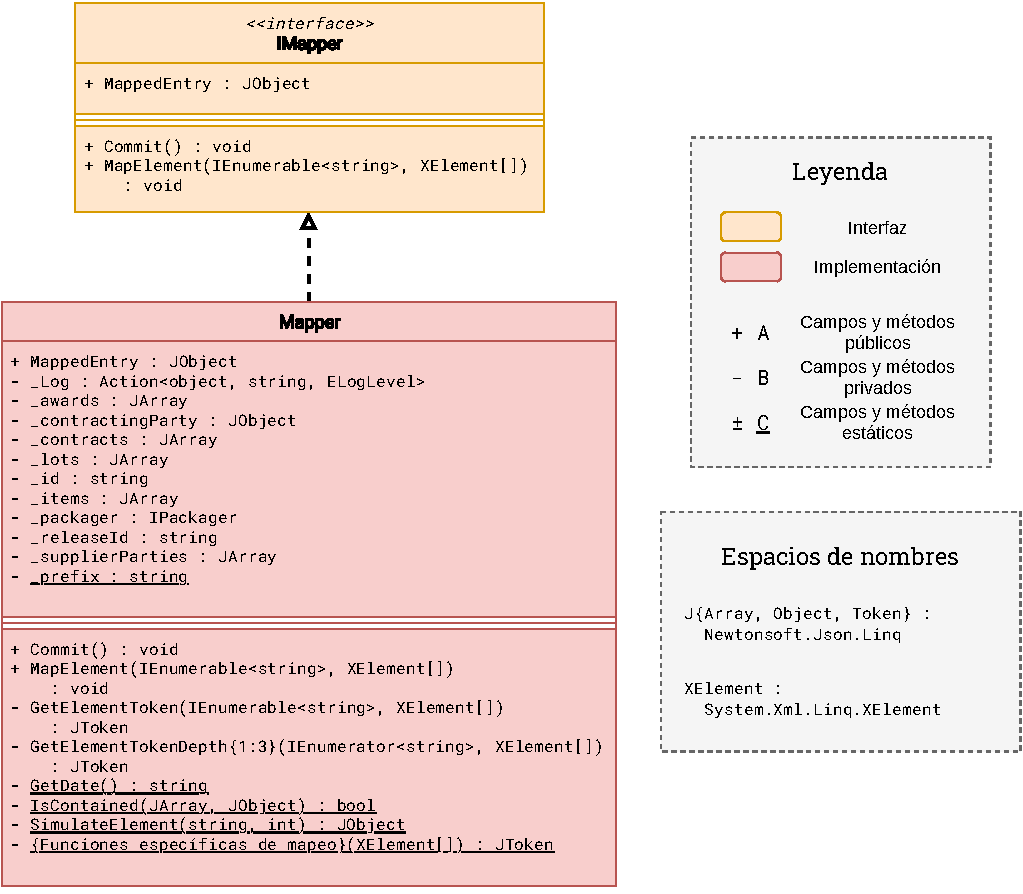
\includegraphics[]{mapper.pdf}
                \captionof{figure}{Diagrama \texttt{UML} del componente \textit{Mapper}}
                \label{fig:mapper}
            \end{figure}
            
            \paragraph{Caso de uso I: mapeado unitario de elementos} \mbox{}\\
                El componente de mapeado de datos debe ser capaz de realizar mapeados unitarios de elementos extraídos de los documentos de licitaciones (esquema \texttt{CODICE}) al esquema \texttt{OCDS}. Para ello, al componente se le indicará tanto el elemento a procesar como la ruta en la que debe almacenar el resultado.
                
            \paragraph{Caso de uso II: mapeado múltiple de elementos} \mbox{}\\
                El componente de mapeado de datos debe ser capaz de realizar mapeados múltiples de elementos siempre y cuando no pueda realizar mapeados unitarios de dichos elementos. Para ello, al componente se le proveera un conjunto de elementos emparentados de la forma más próxima posible. Cuando finalice la ejecución del mapeado, el componente deberá persistir las estructuras de datos en el objeto final para su posterior empaquetado.
                
\newpage
        \subsubsection{Casos de uso del componente de empaquetado de datos}
    
            \begin{figure}[h]
                \centering
                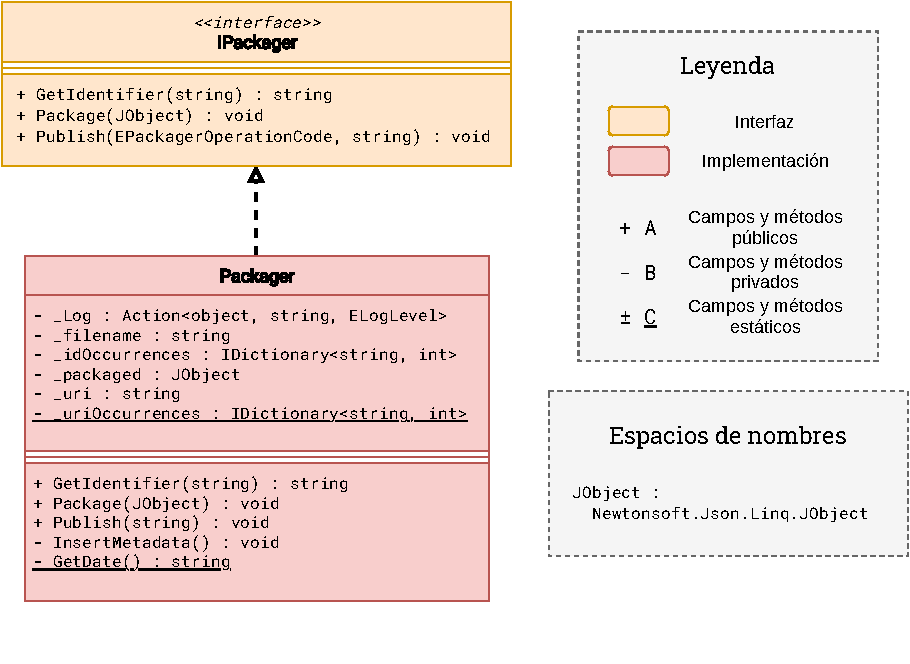
\includegraphics[]{packager.pdf}
                \captionof{figure}{Diagrama \texttt{UML} del componente \textit{Packager}}
                \label{fig:packager}
            \end{figure}
            
            \paragraph{Caso de uso I: empaquetado} \mbox{}\\
                El componente de empaquetado de datos debe ser capaz de recopilar las entradas de los documentos procesados que le lleguen por parte de otros componentes del sistema para persistirlos en un fichero de manera local.
                
            \paragraph{Caso de uso II: evitar colisiones} \mbox{}\\
                El componente de empaquetado de datos debe ser capaz de almacenar temporalmente los identificadores tanto de los propios documentos de licitaciones como de elementos concretos de cada entrada para así evitar colisiones de identificadores no únicos.
        
    \subsection{Trazabilidad de requisitos} \label{subsec:trazabilidad}
        \begin{longtable}{|| M{3cm} | M{12cm} ||} 
                \hline
                    Código del requisito & Ruta del elemento de prueba \\
                \hline\hline
                    \texttt{\textit{RF-1}} & \texttt{UnitTests.ProviderTests.\textit{TestConstructor\{1:4\}}} \\ 
                \hline
                    \texttt{\textit{RF-2}} & \texttt{UnitTests.ProviderTests.\textit{TestConstructor1}} \\
                \hline
                    \texttt{\textit{RF-3}} & \texttt{UnitTests.ProviderTests.\textit{TestConstructor\{2:3\}}} \\
                \hline
                    \texttt{\textit{RF-4}} & \texttt{UnitTests.ProviderTests.\textit{TestConstructor4}} \\
                \hline
                    Código del requisito & Ruta del elemento de prueba \\
                \hline
                \hline
                    \texttt{\textit{RF-5}} & \texttt{UnitTests.ProviderTests.\textit{TestTakeFile\{1:2\}}} \\
                \hline
                    \texttt{\textit{RF-6}} & \texttt{UnitTests.ProviderTests.\textit{TestRemoveFile\{1:2\}}} \\
                \hline
                    \texttt{\textit{RF-7}} & \texttt{UnitTests.ParserTests.\textit{TestGetNamespaces}} \\
                \hline
                    \texttt{\textit{RF-8}} & \texttt{IntegrationTests.\textit{TestProviderParser}} \\
                \hline
                    \texttt{\textit{RF-9}} & \texttt{IntegrationTests.ParserTests.\textit{TestGetEntrySet}} \\
                \hline
                    \texttt{\textit{RF-10}} & \texttt{IntegrationTests.ParserTests.\textit{TestSetEntryRootElement1}} \\
                \hline
                    \texttt{\textit{RF-11}} & \texttt{IntegrationTests.ParserTests.\textit{TestSetEntryRootElement2}} \\
                \hline
                    \texttt{\textit{RF-12}} & \texttt{IntegrationTests.ParserTests.\textit{TestGetElements1}} \\
                \hline
                    \texttt{\textit{RF-13}} & \texttt{IntegrationTests.ParserTests.\textit{TestGetElements2}} \\
                \hline
                    \texttt{\textit{RF-14}} & \texttt{UnitTests.ParserTests.\textit{TestGetNextFile\{1:2\}}} \\
                \hline
                    \texttt{\textit{RF-15}} & \texttt{IntegrationTests.ParserTests.\textit{TestGetSpecificElement}} \\
                \hline
                    \texttt{\textit{RF-16}} & \texttt{UnitTests.ParserTests.\textit{TestGetCodeValue}} \\
                \hline
                    \texttt{\textit{RF-17}} & \texttt{UnitTests.MapperTests.\textit{TestConstructor}} \\
                \hline
                    \texttt{\textit{RF-18}} & \texttt{UnitTests.MapperTests.\textit{TestMapElement1}} \\
                \hline
                    \texttt{\textit{RF-19}} & \texttt{UnitTests.MapperTests.\textit{TestMapElement2}} \\
                \hline
                    \texttt{\textit{RF-20}} & \texttt{UnitTests.MapperTests.\textit{TestMapElement3}} \\
                \hline
                    \texttt{\textit{RF-21}} & \texttt{IntegrationTests.MapperTests.\textit{TestCommit}} \\
                \hline
                    \texttt{\textit{RF-22}} & \texttt{UnitTests.MapperTests.\textit{TagTests}} \\
                \hline
                    \texttt{\textit{RF-23}} & \texttt{UnitTests.MapperTests.\textit{OCIDTests}} \\
                \hline
                    \texttt{\textit{RF-24}} & \texttt{UnitTests.MapperTests.\textit{TenderTitleTests}} \\
                \hline
                    \texttt{\textit{RF-25}} & \texttt{UnitTests.MapperTests.\textit{TenderValueTests}} \\
                \hline
                    \texttt{\textit{RF-26}} & \texttt{UnitTests.MapperTests.\textit{BudgetAmountTests}} \\
                \hline
                    \texttt{\textit{RF-27}} & \texttt{UnitTests.MapperTests.\textit{TenderPeriodStartDateTests}} \\
                \hline
                    \texttt{\textit{RF-28}} & \texttt{UnitTests.MapperTests.\textit{TenderPeriodEndDateTests}} \\
                \hline
                    \texttt{\textit{RF-29}} & \texttt{UnitTests.MapperTests.\textit{TenderPeriodDurationInDaysTests}} \\
                \hline
                    \texttt{\textit{RF-30}} & \texttt{UnitTests.MapperTests.\textit{TenderMainProcurementCategoryTests}} \\
                \hline
                    \texttt{\textit{RF-31}} & \texttt{UnitTests.MapperTests.\textit{TenderLotsIdTests}} \\
                \hline
                    \texttt{\textit{RF-32}} & \texttt{UnitTests.MapperTests.\textit{TenderLotsValueTests}} \\
                \hline
                    \texttt{\textit{RF-33}} & \texttt{UnitTests.MapperTests.\textit{TenderItemsClassificationTests}} \\
                \hline
                    \texttt{\textit{RF-34}} & \texttt{UnitTests.MapperTests.\textit{TenderProcurementMethodTests}} \\
                \hline
                    \texttt{\textit{RF-35}} & \texttt{UnitTests.MapperTests.\textit{TenderProcurementMethodDetailsTests}} \\
                \hline
                    \texttt{\textit{RF-36}} & \texttt{UnitTests.MapperTests.\textit{TenderSubmissionMethodTests}} \\
                \hline
                    \texttt{\textit{RF-37}} & \texttt{UnitTests.MapperTests.\textit{TenderSubmissionMethodDetailsTests}} \\
                \hline
                    \texttt{\textit{RF-38}} & \texttt{UnitTests.MapperTests.\textit{TenderSubmissionMethodTests}} \\
                \hline
                \hline
                    Código del requisito & Ruta del elemento de prueba \\
                \hline
                    \texttt{\textit{RF-39}} & \texttt{UnitTests.MapperTests.\textit{PartiesNameTests}} \\
                \hline
                    \texttt{\textit{RF-40}} & \texttt{UnitTests.MapperTests.\textit{PartiesIdentifierTests}} \\
                \hline
                    \texttt{\textit{RF-41}} & \texttt{UnitTests.MapperTests.\textit{PartiesFieldsTests}} \\
                \hline
                    \texttt{\textit{RF-42}} & \texttt{UnitTests.MapperTests.\textit{AwardIdTests}} \\
                \hline
                    \texttt{\textit{RF-43}} & \texttt{UnitTests.MapperTests.\textit{AwardStatusTests}} \\
                \hline
                    \texttt{\textit{RF-44}} & \texttt{UnitTests.MapperTests.\textit{AwardSupplierTests}} \\
                \hline
                    \texttt{\textit{RF-45}} & \texttt{UnitTests.MapperTests.\textit{AwardValueTests}} \\
                \hline
                    \texttt{\textit{RF-46}} & \texttt{UnitTests.MapperTests.\textit{TenderNumberOfTenderersTests}} \\
                \hline
                    \texttt{\textit{RF-47}} & \texttt{UnitTests.MapperTests.\textit{AwardDateTests}} \\
                \hline
                    \texttt{\textit{RF-48}} & \texttt{UnitTests.MapperTests.\textit{AwardDescriptionTests}} \\
                \hline
                    \texttt{\textit{RF-49}} & \texttt{UnitTests.MapperTests.\textit{ContractIdTests}} \\
                \hline
                    \texttt{\textit{RF-50}} & \texttt{UnitTests.MapperTests.\textit{ContractPeriodStartDateTests}} \\
                \hline
                    \texttt{\textit{RF-51}} & \texttt{UnitTests.PackagerTests.\textit{TestGetIdentifier}} \\
                \hline
                    \texttt{\textit{RF-52}} & \texttt{UnitTests.PackagerTests.\textit{TestPackage}} \\
                \hline
                    \texttt{\textit{RF-53}} & \texttt{UnitTests.PackagerTests.\textit{TestPublish}} \\
                \hline
                    \texttt{\textit{RF-54}} & \texttt{IntegrationTests.ProgramTests.\textit{TestProgram\{1:3\}}} \\
                \hline
                    \texttt{\textit{RF-55}} & \texttt{IntegrationTests.ProgramTests.\textit{TestProgram4}} \\
                \hline
        \end{longtable}
        \addtocounter{table}{-1}
        \captionof{table}{Tabla de trazabilidad de requisitos}
        
    \vspace{1cm}
    
    \subsection{Flujo de ejecución} \label{subsec:flujo}
        
        \begin{figure}[!htb]
            \centering
            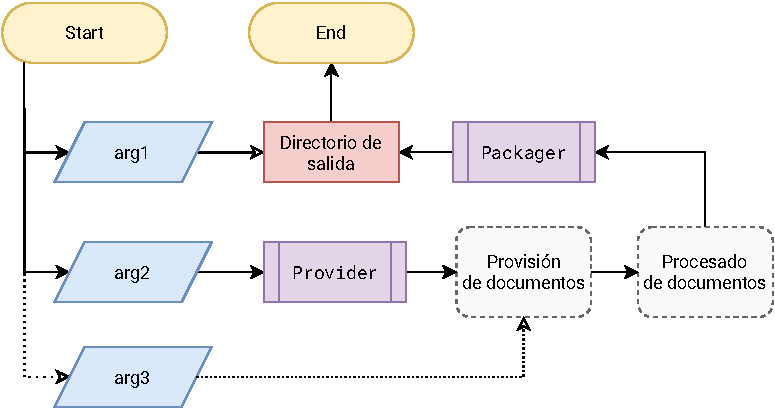
\includegraphics[width=0.825\textwidth]{main_flow.pdf}
            \captionof{figure}{Flujo de ejecución general de la aplicación}
            \label{fig:mainflow}
        \end{figure}
        
        \noindent En la \hyperref[fig:mainflow]{figura 17} se puede apreciar la representación del flujo principal de la aplicación \textit{OCDS\_Mapper}. En primer lugar, cabe destacar la presencia de dos argumentos obligatorios, siendo el primero la ruta del directorio de salida de los ficheros que se generen, y el segundo el descriptor del modo de operación que se pretende ejecutar.
        \\ \\
        En las dos siguientes figuras se detallan los flujos de ejecución correspondientes a la provisión y al procesado de documentos, con el objetivo de simplificar y hacer más clara la representación del funcionamiento del programa.
        
        \begin{figure}[!htb]
            \centering
            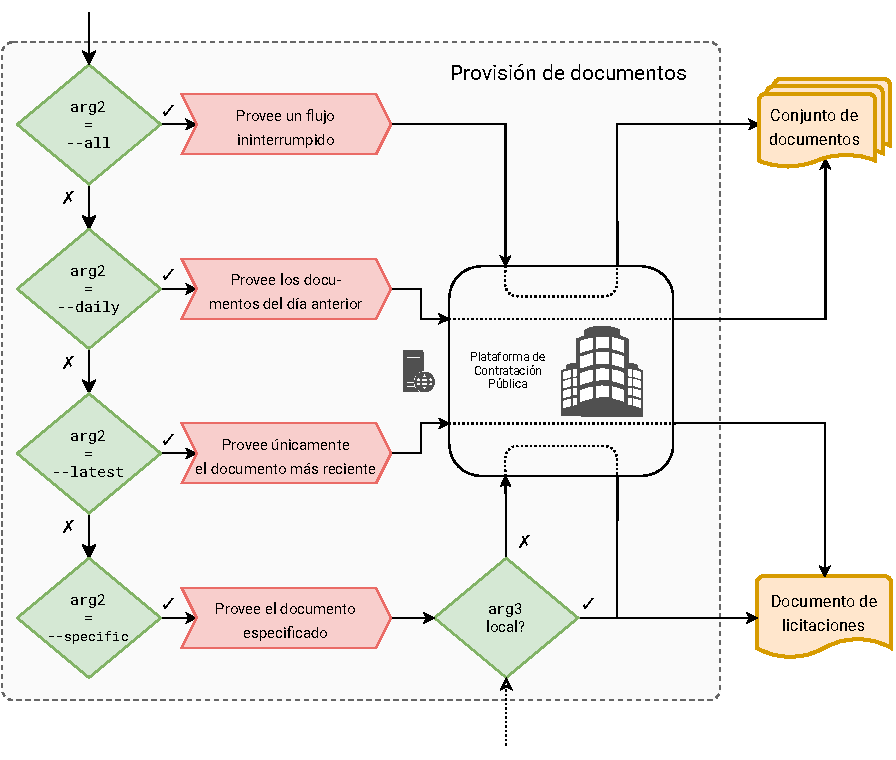
\includegraphics[width=\textwidth]{provider_flow.pdf}
            \captionof{figure}{Flujo de ejecución de la provisión de documentos}
            \label{fig:providerflow}
        \end{figure}
        
        \noindent Mediante la representación del flujo de provisión de documentos se se pueden apreciar los distintos modos de operación del sistema, detallados en secciones previas. Los modos \texttt{--all} y \texttt{--daily} proveen un conjunto de documentos, mientras que los otros dos modos, \texttt{--latest} y \texttt{--specific} proveen un único documento.
        \\ \\
        Este último modo, además, es el único que no accede a la Plataforma de Contratación Pública para descargar documentos si la ruta provista coincide con un archivo local.
        
    \vspace{3cm}
        
        \begin{figure}[!htb]
            \centering
            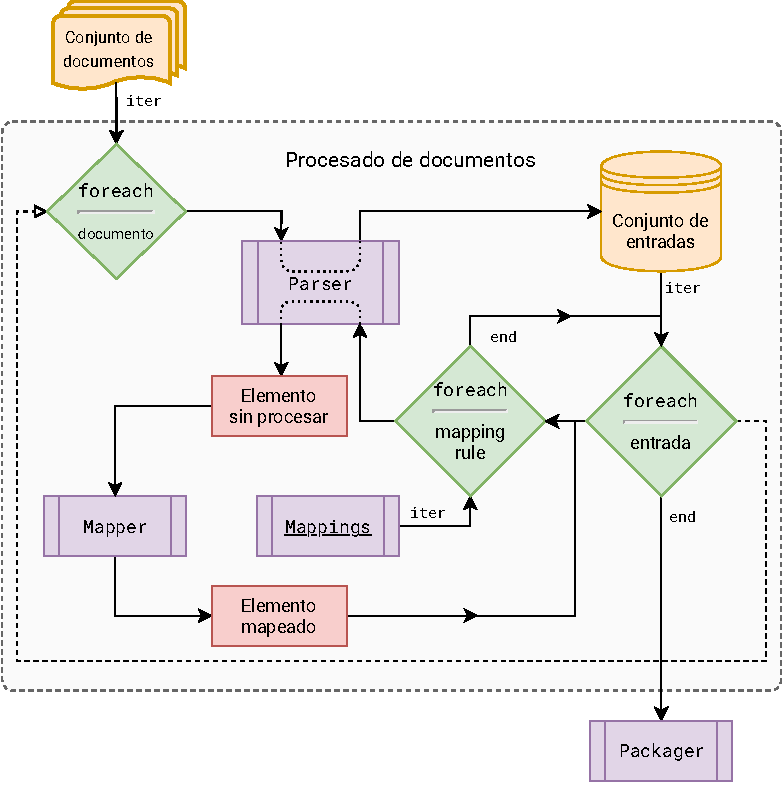
\includegraphics[width=0.95\textwidth]{process_flow.pdf}
            \captionof{figure}{Flujo de ejecución del procesado de documentos}
            \label{fig:processflow}
        \end{figure}
        
        \noindent Para la representación del flujo de procesado de documentos se ha utilizado como \textit{input} un conjunto de documentos en vez de uno único, dado que éste es el caso general y los modos que proveen un solo documento son un caso particular, siendo el conjunto de longitud 1.
        \\ \\
        Por cada documento de licitaciones, se inicializa un componente de parseo que extrae el conjunto de entradas. El procesamiento se realiza entrada a entrada, y en cada una de ellas se evalúan las reglas de mapeado descritas en la clase estática \textit{Mappings}. Se solicita al componente \textit{Parser} que devuelva el elemento concreto de la entrada descrito por la regla de mapeado siendo evaluada, y es el componente \textit{Mapper} el que realiza la transformación de la información de \texttt{CODICE} a \texttt{OCDS}.
        \\ \\
        Una vez cada documento ha sido completamente procesado al finalizar de iterar el conjunto de entradas del mismo, se llama al componente de empaquetado para persistir el documento mapeado.
        
\newpage
    \subsection{Cobertura de código}
        Con el objetivo de proveer un software de calidad, el sistema desarrollado ha sido analizado mediante la plataforma \textit{SonarQube} \cite{SONARQUBE}, capaz de realizar una evaluación del código fuente de manera estática para obtener métricas que sirvan para mejorar la calidad y la seguridad del sistema siendo desarrollado.
        \\ \\
        
        \begin{figure}[h]
            \centering
            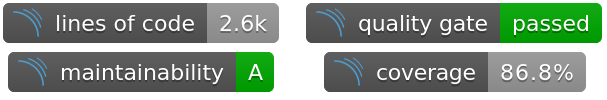
\includegraphics[width=0.625\textwidth]{sonarqube_metrics.png}
            \captionof{figure}{Métricas registradas por \textit{SonarQube}}
            \label{fig:sonarmetrics}
        \end{figure}
        
        \noindent Mediante todos los \textit{tests} descritos en la sección de \hyperref[subsec:trazabilidad]{trazabilidad de requisitos} se ha conseguido una cobertura del código del 86.8\%, sobre las más de 2600 líneas de código de la aplicación. De acuerdo a la \textit{quality gate} por defecto de \textit{SonarQube} para el lenguaje \texttt{C\#}, dicha métrica de cobertura de código es superior al límite (80\%).
        \\ \\
        Entre otras condiciones que se han superado para superar dichas condiciones mínimas, se encuentran la de la duplicidad de líneas (0\%, el límite es 3\%), y los \textit{ratings} de mantenibilidad, fiabilidad y seguridad en calificación \texttt{A}.
        \\ \\
        Se han realizado algunas excepciones al análisis estático del código, cuyas justificaciones se presentan a continuación:
        \begin{itemize}
            \item Regla \texttt{S125}: \textit{"Sections of code should not be commented out"} \cite{SONAR125}. Ignorada debido a que se generaba la alerta en comentarios informativos del funcionamiento de los métodos.
            \item Regla \texttt{S1168}: \textit{"Empty arrays and collections should be returned instead of null"} \cite{SONAR1168}. Ignorada debido a que teniendo el cuenta la implementación del componente \textit{Mapper}, los métodos que no devuelven un objeto \texttt{JObject} devuelven \texttt{null} debido a que el objeto \texttt{JObject} vacío representa un elemento \texttt{JSON} vacío, lo cual no es equivalente a \texttt{null}.
            \item Regla \texttt{S3776}: \textit{"Cognitive Complexity of functions should not be too high"} \cite{SONAR3776}. Por el motivo descrito en el apartado anterior, debido a que cada regla de mapeado está implementada en un sólo método por motivos del modelado del sistema, se ha ignorado esta regla en dichos métodos.
        \end{itemize}
    
\newpage
    \section{Correspondencias entre \texttt{CODICE} y \texttt{OCDS}}

    En esta sección se describirán las correspondencias que se han establecido entre los elementos del estándar \texttt{CODICE} y el estándar \texttt{OCDS}. Dichas correspondencias han sido las implementadas en el \hyperref[sec:software]{software desarrollado}.
    \\ \\
    No todos los elementos de \texttt{CODICE} han sido mapeados, ni todos los campos de \texttt{OCDS} han sido cubiertos, pero sí se han considerado aquellos elementos de mayor interés. Una lista exhaustiva sobre el estado de los elementos puede encontrarse en la siguiente hoja de cálculo \cite{CHECKLIST}.

    \vspace{0.3cm}
    
    \subsection{Datos generales del expediente}
    
    Elementos correspondientes a información genérica del expediente de licitaciones.
    
        \subsubsection{Estado}
            \begin{itemize}
                \item \textbf{Elemento en el esquema \texttt{CODICE}}:
                    \tabto{7.6cm} \texttt{cac-place-ext:ContractFolderStatus/} \\
                    \tabto{7.6cm} \texttt{\textit{cbc-place-ext:ContractFolderStatusCode}}
                \item \textbf{Elemento en el esquema \texttt{OCDS}}:
                    \tabto{7.6cm} \texttt{\textit{tag}}
                \item \textbf{Comentarios}: La lista de posibles códigos del elemento en \texttt{CODICE} se encuentra en el siguiente enlace \cite{CR1}.
                    La lista análoga de códigos en el esquema \texttt{OCDS} se puede consultar en el siguiente enlace \cite{CR2}.
                    La correspondencia entre ambas listas de códigos se ha establecido de la siguiente manera:
                        \subitem - \texttt{PRE} (Anuncio previo) $\rightarrow$ \texttt{planning}
                        \subitem - \texttt{PUB} (En plazo) $\rightarrow$ \texttt{tender}
                        \subitem - \texttt{EV} (Pendiente de adjudicación) $\rightarrow$ \texttt{tender}
                        \subitem - \texttt{ADJ} (Adjudicada) $\rightarrow$ \texttt{award}
                        \subitem - \texttt{RES} (Resuelta) $\rightarrow$ \texttt{contract}
                        \subitem - \texttt{ANUL} (Anulada) $\rightarrow$ \texttt{awardCancellation}
            \end{itemize}
        
        \subsubsection{Número de expediente}
            \begin{itemize}
                \item \textbf{Elemento en el esquema \texttt{CODICE}}:
                    \tabto{7.6cm} \texttt{cac-place-ext:ContractFolderStatus/} \\
                    \tabto{7.6cm} \texttt{\textit{cbc:ContractFolderID}}
                \item \textbf{Elemento en el esquema \texttt{OCDS}}:
                    \tabto{7.6cm} \texttt{\textit{ocid}}
                \item \textbf{Comentarios}: En el esquema de \texttt{OCDS}, los procesos de contratación deben identificarse mediante un código unívoco que será idéntico en cualquier posterior entrega del mismo proceso de contratación. Para asegurar que dichos códigos no puedan colisionar, \texttt{OCDS} provee a los publicadores prefijos que concatenar a los identificadores internos para así asegurar la creación de identificadores globales únicos.
            \end{itemize}
        
        \subsubsection{Objeto del contrato}
            \begin{itemize}
                \item \textbf{Elemento en el esquema \texttt{CODICE}}:
                    \tabto{7.6cm} \texttt{cac-place-ext:ContractFolderStatus/} \\
                    \tabto{7.6cm} \texttt{cac:ProcurementProject/} \\
                    \tabto{7.6cm} \texttt{\textit{cbc:Name}}
                \item \textbf{Elemento en el esquema \texttt{OCDS}}:
                    \tabto{7.6cm} \texttt{tender.\textit{title}}
            \end{itemize}
        
        \subsubsection{Valor estimado e importe de licitación}
            \begin{itemize}
                \item \textbf{Elementos en el esquema \texttt{CODICE}}:
                    \tabto{7.7cm} \texttt{cac-place-ext:ContractFolderStatus/} \\
                    \tabto{7.7cm} \texttt{cac:ProcurementProject/} \\
                    \tabto{7.7cm} \texttt{cac:BudgetAmount/} \\
                    \tabto{7.7cm} \{\texttt{\textit{cbc:EstimatedOverallContractAmount}}, \\
                    \tabto{7.7cm} \texttt{\textit{cbc:TotalAmount}}\}
                \item \textbf{Elementos en el esquema \texttt{OCDS}}:
                    \tabto{7.7cm} \texttt{EstimatedOverallContractAmount} \\ \tabto{8cm} $\rightarrow$ \texttt{tender.\textit{value}} \\
                    \tabto{7.7cm} \texttt{TotalAmount} \\ \tabto{8cm} $\rightarrow$ \texttt{planning.budget.\textit{amount}}
            \end{itemize}
        
        \subsubsection{Duración del contrato}
            \begin{itemize}
                \item \textbf{Elementos en el esquema \texttt{CODICE}}:
                    \tabto{7.7cm} \texttt{cac-place-ext:ContractFolderStatus/} \\
                    \tabto{7.7cm} \texttt{cac:ProcurementProject/} \\
                    \tabto{7.7cm} \texttt{cac:PlannedPeriod/} \\
                    \tabto{7.7cm} \{\texttt{\textit{cbc:StartDate}}, \\
                    \tabto{7.7cm} \{\texttt{\textit{cbc:EndDate}}, \\
                    \tabto{7.7cm} \texttt{\textit{cbc:DurationMeasure}}\}\}
                \item \textbf{Elementos en el esquema \texttt{OCDS}}:
                    \tabto{7.7cm} \texttt{StartDate} \\ \tabto{8cm} $\rightarrow$ \texttt{tender.tenderPeriod.\textit{startDate}} \\
                    \tabto{7.7cm} \texttt{EndDate} \\ \tabto{8cm} $\rightarrow$ \texttt{tender.tenderPeriod.\textit{endDate}}
                    \tabto{7.7cm} \texttt{DurationMeasure} \\ \tabto{8cm} $\rightarrow$ \texttt{tender.tenderPeriod.\textit{durationInDays}}
                \item \textbf{Comentarios}: La duración prevista del contrato puede expresarse mediante una fecha de inicio y una de final, o bien mediante una fecha de inicio y una duración prevista, cuyos valores pueden ser expresados mediante días (\texttt{DAY}), meses (\texttt{MON}) o años (\texttt{ANN}).
            \end{itemize}
        
        \subsubsection{Tipo de contrato}
            \begin{itemize}
                \item \textbf{Elemento en el esquema \texttt{CODICE}}:
                    \tabto{7.6cm} \texttt{cac-place-ext:ContractFolderStatus/} \\
                    \tabto{7.6cm} \texttt{cac:ProcurementProject/} \\
                    \tabto{7.6cm} \texttt{\textit{cbc:TypeCode}}
                \item \textbf{Elemento en el esquema \texttt{OCDS}}:
                    \tabto{7.6cm} \texttt{tender.\textit{mainProcurementCategory}}
                \item \textbf{Comentarios}: La lista de posibles valores que pueden tomar los códigos que describen los tipos de contrato en \texttt{CODICE} pueden encontrarse en el siguiente enlace \cite{CR3}. La lista análoga de códigos en el esquema \texttt{OCDS} se puede consultar en el siguiente enlace \cite{CR4}. La correspondencia entre ambas listas de códigos se ha establecido de la siguiente manera:
                        \subitem - \texttt{1} (Suministros) $\rightarrow$ \texttt{goods}
                        \subitem - \texttt{2} (Servicios) $\rightarrow$ \texttt{services}
                        \subitem - \texttt{3} (Obras) $\rightarrow$ \texttt{works}
                        \subitem - \texttt{21} (Gestión de servicios públicos) $\rightarrow$ \texttt{services}
                        \subitem - \texttt{22} (Gestión de servicios) $\rightarrow$ \texttt{services}
                        \subitem - \texttt{31} (Concesión de obras públicas) $\rightarrow$ \texttt{works}
                        \subitem - \texttt{32} (Concesión de obras) $\rightarrow$ \texttt{works}
            \end{itemize}
        
        \subsubsection{Enlaces de descarga de pliegos}
            \begin{itemize}
                \item \textbf{Elementos en el esquema \texttt{CODICE}}:
                    \tabto{7.7cm} \texttt{cac-place-ext:ContractFolderStatus/} \\
                    \tabto{7.7cm} \{\texttt{cac:LegalDocumentReference/}, \\
                    \tabto{7.7cm} \texttt{cac:TechnicalDocumentReference/}, \\
                    \tabto{7.7cm} \texttt{cac:AdditionalDocumentReference/}\} \\
                    \tabto{7.7cm} \texttt{\textit{cbc:ID}},\\
                    \tabto{7.7cm} \texttt{cac:Attachment/} \\
                    \tabto{7.7cm} \texttt{cac:ExternalReference/} \\
                    \tabto{7.7cm} \texttt{\textit{cbc:URI}}
                \item \textbf{Elemento en el esquema \texttt{OCDS}}:
                    \tabto{7.7cm} \texttt{tender.\textit{documents}}
                \item \textbf{Comentarios}: Los distintos pliegos que pueden documentar un proceso de contratación vienen descritos, en su tipo, por el elemento inmediatamente inferior a \texttt{ContractFolderStatus}, y su mapeo al esquema \texttt{OCDS} se representa mediante la lista de códigos documentType \cite{CR5}.
                        \subitem - LegalDocumentReference $\rightarrow$ \texttt{?}
                        \subitem - TechnicalDocumentReference $\rightarrow$ \texttt{technicalSpecifications}
                        \subitem - AdditionalDocumentReference $\rightarrow$ \texttt{?}
            \end{itemize}

    \vspace{0.3cm}
    
    \subsection{Lotes}
        
        El uso de lotes en el esquema \texttt{OCDS} viene otorgado por la extensión de mismo nombre \cite{CR6}.
    
        \subsubsection{Número de lote}
            \begin{itemize}
                \item \textbf{Elemento en el esquema \texttt{CODICE}}:
                    \tabto{7.6cm} \texttt{cac-place-ext:ContractFolderStatus/} \\
                    \tabto{7.6cm} \texttt{cac:ProcurementProjectLot/} \\
                    \tabto{7.6cm} \texttt{\textit{cbc:ID}}
                \item \textbf{Elementos en el esquema \texttt{OCDS}}:
                    \tabto{7.6cm} \texttt{tender.lots[i].\textit{id}} \\
                    \tabto{7.6cm} \texttt{tender.items[i].\textit{id}} \\
                    \tabto{7.6cm} \texttt{tender.items[i].\textit{relatedLot}} \\
                \item \textbf{Comentarios}: En todos los apartados de esta sección se utilizará la notación \texttt{lots[i]} e \texttt{items[i]} para referirse a los i-ésimos objetos representando el lote y el artículo, respectivamente, dentro de las colecciones de éstos. El campo \texttt{relatedLot} se utilizará para enlazar el artículo con su lote.
            \end{itemize}
            
        \subsubsection{Objeto del lote}
            \begin{itemize}
                \item \textbf{Elemento en el esquema \texttt{CODICE}}:
                    \tabto{7.6cm} \texttt{cac-place-ext:ContractFolderStatus/} \\
                    \tabto{7.6cm} \texttt{cac:ProcurementProjectLot/} \\
                    \tabto{7.6cm} \texttt{cac:ProcurementProject/} \\
                    \tabto{7.6cm} \texttt{\textit{cbc:Name}}
                \item \textbf{Elemento en el esquema \texttt{OCDS}}:
                    \tabto{7.6cm} \texttt{tender.lots[i].\textit{name}}
            \end{itemize}
        
        \subsubsection{Importe del lote}
            \begin{itemize}
                \item \textbf{Elemento en el esquema \texttt{CODICE}}:
                    \tabto{7.6cm} \texttt{cac-place-ext:ContractFolderStatus/} \\
                    \tabto{7.6cm} \texttt{cac:ProcurementProjectLot/} \\
                    \tabto{7.6cm} \texttt{cac:ProcurementProject/} \\
                    \tabto{7.6cm} \texttt{cac:BudgetAmount/} \\
                    \tabto{7.6cm} \texttt{\textit{cbc:TotalAmount}}
                \item \textbf{Elemento en el esquema \texttt{OCDS}}:
                    \tabto{7.6cm} \texttt{tender.lots[i].\textit{value}}
            \end{itemize}
            
        \subsubsection{Clasificación \texttt{CPV}}
            \begin{itemize}
                \item \textbf{Elemento en el esquema \texttt{CODICE}}:
                    \tabto{7.6cm} \texttt{cac-place-ext:ContractFolderStatus/} \\
                    \tabto{7.6cm} \texttt{cac:ProcurementProjectLot/} \\
                    \tabto{7.6cm} \texttt{cac:ProcurementProject/} \\
                    \tabto{7.6cm} \texttt{cac:RequiredCommodityClassification/} \\
                    \tabto{7.6cm} \texttt{\textit{cbc:ItemClassificationCode}}
                \item \textbf{Elemento en el esquema \texttt{OCDS}}:
                    \tabto{7.6cm} \texttt{tender.lots[i].\textit{classification}}
                \item \textbf{Comentarios}: El sistema de clasificación de bienes y servicios utilizado en \texttt{CODICE}, \texttt{CPV} \cite{CR7}, es un estándar válido en \texttt{OCDS}, indicándolo en el campo \texttt{classification.\textit{schema}}.
            \end{itemize}

    \vspace{0.3cm}

    \subsection{Procesos de licitación}
    
        Elementos correspondientes a los procedimientos de contratación.
    
        \subsubsection{Tipo de procedimiento}
            \begin{itemize}
                \item \textbf{Elemento en el esquema \texttt{CODICE}}:
                    \tabto{7.6cm} \texttt{cac-place-ext:ContractFolderStatus/} \\
                    \tabto{7.6cm} \texttt{cac:TenderingProcess/} \\
                    \tabto{7.6cm} \texttt{\textit{cbc:ProcedureCode}}
                \item \textbf{Elemento en el esquema \texttt{OCDS}}:
                    \tabto{7.6cm} \texttt{tender.\textit{procurementMethod}}
                \item \textbf{Comentarios}: La lista de posibles códigos del elemento en \texttt{CODICE} se encuentra en el siguiente enlace \cite{CR8}.
                    La lista análoga de códigos en el esquema \texttt{OCDS} se puede consultar en el siguiente enlace \cite{CR9}.
                    La correspondencia entre ambas listas de códigos se ha establecido de la siguiente manera:
                        \subitem - \texttt{1} (Abierto) $\rightarrow$ \texttt{open}
                        \subitem - \texttt{2} (Restringido) $\rightarrow$ \texttt{selective}
                        \subitem - \texttt{3} (Negociado sin publicidad) $\rightarrow$ \texttt{limited}
                        \subitem - \texttt{4} (Negociado con publicidad) $\rightarrow$ \texttt{limited}
                        \subitem - \texttt{5} (Diálogo competitivo) $\rightarrow$ \texttt{open}
                        \subitem - \texttt{6} (Contrato menor) $\rightarrow$ \texttt{open}
                        \subitem - \texttt{7} (Derivado de acuerdo macro) $\rightarrow$ \texttt{selective}
                        \subitem - \texttt{8} (Concurso de proyectos) $\rightarrow$ \texttt{open}
                        \subitem - \texttt{9} (Abierto simplificado) $\rightarrow$ \texttt{open}
                        \subitem - \texttt{10} (Asociación para la innovación) $\rightarrow$ \texttt{limited}
                        \subitem - \texttt{11} (Derivado de asociación para la innovación) $\rightarrow$ \texttt{limited}
                        \subitem - \texttt{12} (Basado en un sistema dinámico de adquisición) $\rightarrow$ \texttt{open}
                        \subitem - \texttt{13} (Licitación con negociación) $\rightarrow$ \texttt{open}
                        \subitem - \texttt{100} (Normas internas) $\rightarrow$ \texttt{limited}
            \end{itemize}
        
        \subsubsection{Sistema de contratación} \label{subsubsec:SistemaDeContratacion}
            \begin{itemize}
                \item \textbf{Elemento en el esquema \texttt{CODICE}}:
                    \tabto{7.6cm} \texttt{cac-place-ext:ContractFolderStatus/} \\
                    \tabto{7.6cm} \texttt{cac:TenderingProcess/} \\
                    \tabto{7.6cm} \texttt{\textit{cbc:ContractingSystemCode}}
                \item \textbf{Elemento en el esquema \texttt{OCDS}}:
                    \tabto{7.6cm} \texttt{tender.\textit{procurementMethodDetails\_es}}
                \item \textbf{Comentarios}: Este elemento describe si el sistema de contratación se trata de un contrato, de un acuerdo marco, o de un sistema dinámico de adquisición. Con el sufijo \texttt{es} se especifica que el campo muestra su información en castellano, tal y como aparece en el documento de códigos \cite{CR10} de \texttt{CODICE}.
            \end{itemize}
        
        \subsubsection{Presentación de la oferta} \label{subsec:PresentacionOferta}
            \begin{itemize}
                \item \textbf{Elemento en el esquema \texttt{CODICE}}:
                    \tabto{7.6cm} \texttt{cac-place-ext:ContractFolderStatus/} \\
                    \tabto{7.6cm} \texttt{cac:TenderingProcess/} \\
                    \tabto{7.6cm} \texttt{\textit{cbc:SubmissionMethodCode}}
                \item \textbf{Elemento en el esquema \texttt{OCDS}}:
                    \tabto{7.6cm} \texttt{tender.\textit{submissionMethod}}
                \item \textbf{Comentarios}: La lista de posibles códigos del elemento en \texttt{CODICE} se encuentra en el siguiente enlace \cite{CR11}.
                    La lista análoga de códigos en el esquema \texttt{OCDS} se puede consultar en el siguiente enlace \cite{CR12}.
                    La correspondencia entre ambas listas de códigos se ha establecido de la siguiente manera:
                        \subitem - \texttt{1} (Electrónica) $\rightarrow$ \texttt{[electronicSubmission]}
                        \subitem - \texttt{2} (Manual) $\rightarrow$ \texttt{[written]}
                        \subitem - \texttt{3} (Manual y/o Electrónica) $\rightarrow$ \texttt{[electronicSubmission, written]}
            \end{itemize}
        
        \subsubsection{Idioma de presentación de la oferta}
            \begin{itemize}
                \item \textbf{Elemento en el esquema \texttt{CODICE}}:
                    \tabto{7.6cm} \texttt{cac-place-ext:ContractFolderStatus/} \\
                    \tabto{7.6cm} \texttt{cac:TenderingTerms/} \\
                    \tabto{7.6cm} \texttt{cac:Language/} \\
                    \tabto{7.6cm} \texttt{\textit{cbc:ID}}
                \item \textbf{Elemento en el esquema \texttt{OCDS}}:
                    \tabto{7.6cm} \texttt{tender.\textit{submissionMethodDetails}}
            \end{itemize}
        
        \subsubsection{Licitación son subasta electrónica}
            \begin{itemize}
                \item \textbf{Elemento en el esquema \texttt{CODICE}}:
                    \tabto{7.6cm} \texttt{cac-place-ext:ContractFolderStatus/} \\
                    \tabto{7.6cm} \texttt{cac:TenderingProcess/} \\
                    \tabto{7.6cm} \texttt{cac:AuctionTerms/} \\
                    \tabto{7.6cm} \texttt{\textit{cbc:AuctionConstraintIndicator}}
                \item \textbf{Elemento en el esquema \texttt{OCDS}}:
                    \tabto{7.6cm} \texttt{tender.\textit{submissionMethod}}
                \item \textbf{Comentarios}: Si en el elemento \texttt{AuctionConstraintIndicator} está indicado el valor \texttt{true}, significa que la licitación estará sujeta a subasta electrónica, por lo que el valor \texttt{electronicAuction} de la lista de códigos \texttt{submissionMethod} \cite{CR11} se sobreescribe en el campo \texttt{tender.submissionMethod}, que ya había sido inicializado por el elemento \hyperref[subsec:PresentacionOferta]{Presentación de la oferta}.
            \end{itemize}
        
    \vspace{0.3cm}
    
    \subsection{Entidades adjudicadoras}
    
        Elementos correspondientes a información acerca de los adjudicadores.
    
        \subsubsection{Órgano de contratación}
            \begin{itemize}
                \item \textbf{Elemento en el esquema \texttt{CODICE}}:
                    \tabto{7.6cm} \texttt{cac-place-ext:ContractFolderStatus/} \\
                    \tabto{7.6cm} \texttt{cac-place-ext:LocatedContractingParty/} \\
                    \tabto{7.6cm} \texttt{cac:Party/} \\
                    \tabto{7.6cm} \texttt{cac:PartyName/} \\
                    \tabto{7.6cm} \texttt{\textit{cbc:Name}}
                \item \textbf{Elemento en el esquema \texttt{OCDS}}:
                    \tabto{7.6cm} \texttt{parties[i].\textit{name}}
                \item \textbf{Comentarios}: En todos los apartados de esta sección se utilizará la notación \texttt{parties[i]} para referirse al mismo objeto representando a la entidad adjudicadora, debido a que \texttt{parties} es una colección de objetos representando a todas las partes involucradas.
            \end{itemize}
        
        \subsubsection{Ubicación orgánica} \label{subsec:UbicacionOrganica}
            \begin{itemize}
                \item \textbf{Elemento en el esquema \texttt{CODICE}}:
                    \tabto{7.6cm} \texttt{cac-place-ext:ContractFolderStatus/} \\
                    \tabto{7.6cm} \texttt{cac-place-ext:LocatedContractingParty/} \\
                    \tabto{7.6cm} \texttt{cac:Party/} \\
                    \tabto{7.6cm} \texttt{cac:PartyIdentification/} \\
                    \tabto{7.6cm} \texttt{\textit{cbc:ID}}
                \item \textbf{Elementos en el esquema \texttt{OCDS}}:
                    \tabto{7.6cm} \texttt{parties[i].\textit{id}} \\
                    \tabto{7.6cm} \texttt{parties[i].\textit{identifier.schema}} \\
                    \tabto{7.6cm} \texttt{parties[i].\textit{identifier.id}} \\
                    \tabto{7.6cm} \texttt{parties[i].\textit{additionalIdentifiers}} \\
                    \tabto{7.6cm} \texttt{parties[i].\textit{roles}}
                \item \textbf{Comentarios}: Siguiendo la directriz del estándar \texttt{OCDS} sobre los esquemas de identificación de organizaciones \cite{CR13}, estos elementos se procesan dependiendo de su esquema: \texttt{DIR3} \cite{CR14} o \texttt{NIF} \cite{CR15} (\texttt{RMC}). Adicionalmente, si \texttt{PartyIdentification} contiene ambos identificadores, se utilizará el campo \texttt{additionalIdentifiers} para mapear la máxima cantidad de información. Por último, en este elemento de mapeo se ha añadido el rol de la parte adjudicadora (\texttt{procuringEntity}).
            \end{itemize}
        
        \subsubsection{Otros campos}
            \begin{itemize}
                \item \textbf{Elementos en el esquema \texttt{CODICE}}:
                    \tabto{7.6cm} \texttt{cac-place-ext:ContractFolderStatus/} \\
                    \tabto{7.6cm} \texttt{cac-place-ext:LocatedContractingParty/} \\
                    \tabto{7.6cm} \texttt{cac:Party/} \\
                    \tabto{7.6cm} \texttt{\textit{cac:PostalAddress}} \\
                    \tabto{7.6cm} \texttt{\textit{cac:Contact}} \\
                \item \textbf{Elementos en el esquema \texttt{OCDS}}:
                    \tabto{7.6cm} \texttt{parties[i].\textit{address}} \\
                    \tabto{7.6cm} \texttt{parties[i].\textit{countryName}} \\
                    \tabto{7.6cm} \texttt{parties[i].\textit{contactPoint}}
            \end{itemize}
    
    \vspace{0.3cm}
    
    \subsection{Resultado del procedimiento}
        
        Elementos referidos al resultado de la licitación.
    
        \subsubsection{Identificador}
            \begin{itemize}
                \item \textbf{Elemento en el esquema \texttt{CODICE}}:
                    \tabto{7.6cm} \texttt{cac-place-ext:ContractFolderStatus/} \\
                    \tabto{7.6cm} \texttt{cac:TenderResult/} \\
                    \tabto{7.6cm} \texttt{cac:AwardedTenderedProject/} \\
                    \tabto{7.6cm} \texttt{\textit{cbc:ProcurementProjectLotID}}
                \item \textbf{Elemento en el esquema \texttt{OCDS}}:
                    \tabto{7.6cm} \texttt{awards[i].\textit{id}}
                \item \textbf{Comentarios}: En todos los apartados de esta sección se utilizará la notación \texttt{awards[i]} para referirse al mismo objeto representando el resultado de un procedimiento de adjudicación dentro de un mismo proceso de contratación.
            \end{itemize}
            
        \subsubsection{Resultado}
            \begin{itemize}
                \item \textbf{Elemento en el esquema \texttt{CODICE}}:
                    \tabto{7.6cm} \texttt{cac-place-ext:ContractFolderStatus/} \\
                    \tabto{7.6cm} \texttt{cac:TenderResult/} \\
                    \tabto{7.6cm} \texttt{\textit{cbc:ResultCode}}
                \item \textbf{Elemento en el esquema \texttt{OCDS}}:
                    \tabto{7.6cm} \texttt{awards[i].\textit{status}}
                \item \textbf{Comentarios}: La lista de posibles códigos del elemento en \texttt{CODICE} se encuentra en el siguiente enlace \cite{CR16}.
                    La lista análoga de códigos en el esquema \texttt{OCDS} se puede consultar en el siguiente enlace \cite{CR17}.
                    La correspondencia entre ambas listas de códigos se ha establecido de la siguiente manera:
                        \subitem - \texttt{1} (Adjudicado provisionalmente) $\rightarrow$ \texttt{pending}
                        \subitem - \texttt{2} (Adjudicado definitivamente) $\rightarrow$ \texttt{active}
                        \subitem - \texttt{3} (Desierto) $\rightarrow$ \texttt{cancelled}
                        \subitem - \texttt{4} (Desistimiento) $\rightarrow$ \texttt{unsuccessful}
                        \subitem - \texttt{5} (Renuncia) $\rightarrow$ \texttt{unsuccessful}
                        \subitem - \texttt{6} (Desierto provisionalmente) $\rightarrow$ \texttt{pending}
                        \subitem - \texttt{7} (Desierto definitivamente) $\rightarrow$ \texttt{cancelled}
                        \subitem - \texttt{8} (Adjudicado) $\rightarrow$ \texttt{active}
                        \subitem - \texttt{9} (Formalizado) $\rightarrow$ \texttt{active}
                        \subitem - \texttt{10} (Licitador mejor valorado: requerimiento de documentación) $\rightarrow$ \texttt{active}
            \end{itemize}
            
        \subsubsection{Identidad del adjudicatario}
            \begin{itemize}
                \item \textbf{Elementos en el esquema \texttt{CODICE}}:
                    \tabto{7.6cm} \texttt{cac-place-ext:ContractFolderStatus/} \\
                    \tabto{7.6cm} \texttt{cac:TenderResult/} \\
                    \tabto{7.6cm} \texttt{cac:WinningParty/} \\
                    \tabto{7.7cm} \{\texttt{\textit{cac:PartyIdentification}}, \\
                    \tabto{7.7cm} \texttt{\textit{cac:PartyName}}\}
                \item \textbf{Elementos en el esquema \texttt{OCDS}}:
                    \tabto{7.6cm} \texttt{awards[i].\textit{suppliers}} \\
                    \tabto{7.6cm} \texttt{\textit{parties[j]}}
                \item \textbf{Comentarios}: Debido a que este mapeo introduce en el documento la identidad del adjudicatario, también debe introducir en el campo \texttt{parties} la referencia a dicha parte involucrada. De manera análoga al mapeo que realiza  \hyperref[subsec:UbicacionOrganica]{Ubicación orgánica}, el campo \texttt{identifier} tanto en el campo \texttt{suppliers} como en la colección \texttt{parties} detecta si la identificación de la entidad es del tipo DIR3 o NIF, indicándolo en el campo \texttt{schema}. Por último, este mapeo también introduce en la referencia al adjudicatario en \texttt{parties} en el campo \texttt{roles} el valor \texttt{supplier}, tal y como se indica en la lista de códigos de \texttt{OCDS} sobre roles de las partes involucradas \cite{CR18}.
            \end{itemize}
            
        \subsubsection{Importe de adjudicación}
            \begin{itemize}
                \item \textbf{Elemento en el esquema \texttt{CODICE}}:
                    \tabto{7.6cm} \texttt{cac-place-ext:ContractFolderStatus/} \\
                    \tabto{7.6cm} \texttt{cac:TenderResult/} \\
                    \tabto{7.6cm} \texttt{cac:AwardedTenderedProject/} \\
                    \tabto{7.6cm} \texttt{cac:LegalMonetaryTotal/} \\
                    \tabto{7.6cm} \texttt{\textit{cbc:PayableAmount}}
                \item \textbf{Elemento en el esquema \texttt{OCDS}}:
                    \tabto{7.6cm} \texttt{awards[i].\textit{value}}
            \end{itemize}
            
        \subsubsection{Número de licitadores participantes}
            \begin{itemize}
                \item \textbf{Elemento en el esquema \texttt{CODICE}}:
                    \tabto{7.6cm} \texttt{cac-place-ext:ContractFolderStatus/} \\
                    \tabto{7.6cm} \texttt{cac:TenderResult/} \\
                    \tabto{7.6cm} \texttt{\textit{cbc:ReceivedTenderQuantity}}
                \item \textbf{Elemento en el esquema \texttt{OCDS}}:
                    \tabto{7.6cm} \texttt{tender.\textit{numberOfTenderers}}
                \item \textbf{Comentarios}: Dado que \texttt{OCDS} no provee el campo \texttt{numberOfTenderers} dentro de la colección de \texttt{awards}, este mapeo sólo se realizará en el caso de que el proceso de adjudicación sólo contenga un lote, es decir, la longitud de la colección \texttt{awards} sea 1 y, por tanto, \texttt{numberOfTenderers} refleje efectivamente el número de participantes.
            \end{itemize}
            
        \subsubsection{Fecha de la adjudicación}
            \begin{itemize}
                \item \textbf{Elemento en el esquema \texttt{CODICE}}:
                    \tabto{7.6cm} \texttt{cac-place-ext:ContractFolderStatus/} \\
                    \tabto{7.6cm} \texttt{cac:TenderResult/} \\
                    \tabto{7.6cm} \texttt{\textit{cbc:AwardDate}}
                \item \textbf{Elementos en el esquema \texttt{OCDS}}:
                    \tabto{7.6cm} \texttt{awards[i].\textit{date}}
            \end{itemize}
            
        \subsubsection{Descripción de la adjudicación}
            \begin{itemize}
                \item \textbf{Elemento en el esquema \texttt{CODICE}}:
                    \tabto{7.6cm} \texttt{cac-place-ext:ContractFolderStatus/} \\
                    \tabto{7.6cm} \texttt{cac:TenderResult/} \\
                    \tabto{7.6cm} \texttt{\textit{cbc:Description}}
                \item \textbf{Elemento en el esquema \texttt{OCDS}}:
                    \tabto{7.6cm} \texttt{awards[i].\textit{description\_es}}
                \item \textbf{Comentarios}: Como sucedía en el elemento  \hyperref[subsubsec:SistemaDeContratacion]{sistema de contratación}, se hace uso del sufijo \texttt{es} para indicar que el campo contendrá su información en castellano.
            \end{itemize}
            
    \vspace{0.3cm}
    
    \subsection{Información sobre el contrato}
        
        Elementos relativos a los contratos adjudicados.
    
        \subsubsection{Identificador}
            \begin{itemize}
                \item \textbf{Elemento en el esquema \texttt{CODICE}}:
                    \tabto{7.6cm} \texttt{cac-place-ext:ContractFolderStatus/} \\
                    \tabto{7.6cm} \texttt{cac:TenderResult/} \\
                    \tabto{7.6cm} \texttt{cac:Contract/} \\
                    \tabto{7.6cm} \texttt{\textit{cbc:ID}}
                \item \textbf{Elemento en el esquema \texttt{OCDS}}:
                    \tabto{7.6cm} \texttt{contracts[i].\textit{id}}
                \item \textbf{Comentarios}: En todos los apartados de esta sección se utilizará la notación \texttt{contracts[i]} para referirse al mismo objeto representando un contrato formalizado dentro de un mismo proceso de contratación.
            \end{itemize}
            
        \subsubsection{Fecha de entrada en vigor}
            \begin{itemize}
                \item \textbf{Elemento en el esquema \texttt{CODICE}}:
                    \tabto{7.6cm} \texttt{cac-place-ext:ContractFolderStatus/} \\
                    \tabto{7.6cm} \texttt{cac:TenderResult/} \\
                    \tabto{7.6cm} \texttt{\textit{cbc:StartDate}}
                \item \textbf{Elemento en el esquema \texttt{OCDS}}:
                    \tabto{7.6cm} \texttt{contracts[i].period.\textit{startDate}}
            \end{itemize}
            
\newpage
    \section{Conclusions}

    ...

\newpage
    \section{References}

\begingroup
    \renewcommand{\section}[2]{}%
    \begin{thebibliography}{X}
    
        \bibitem{ID-1}
        \textit{Name book or paper}, Authors, Year.
        
        \bibitem{ID-2}
        \textit{Name book or paper}, Authors, Year.
        
    \end{thebibliography}
\endgroup

\newpage
    \section{Anexos}

    \subsection{Anexo I: Ejemplos de los mapeos entre CODICE y OCDS}

        \subsubsection{Datos generales del expediente}
            \paragraph{Estado} \mbox{}\\
                \begin{lstlisting}[language=lXML]
                    <cac-place-ext:ContractFolderStatus>
                        <cbc-place-ext:ContractFolderStatusCode languageID="es"
                         listURI="https://contrataciondelestado.es/codice/cl/2.04/
                         SyndicationContractFolderStatusCode-2.04.gc">
                            ADJ
                        </cbc-place-ext:ContractFolderStatusCode>
                    </cac-place-ext:ContractFolderStatus>
                \end{lstlisting}
                
                \begin{center}
                    $\big\Downarrow$
                \end{center}
                
                \begin{lstlisting}[language=lJSON]
                    {
                        "tag": [
                            "award"
                        ]
                    }
                \end{lstlisting}
                
            \paragraph{Número de expediente} \mbox{}\\
                \begin{lstlisting}[language=lXML]
                    <cac-place-ext:ContractFolderStatus>
                        <cbc:ContractFolderID>
                            002/2021-CONTR
                        </cbc:ContractFolderID>
                    </cac-place-ext:ContractFolderStatus>
                \end{lstlisting}
                
                \begin{center}
                    $\big\Downarrow$
                \end{center}
                
                \begin{lstlisting}[language=lJSON]
                    {
                        "ocid": "ES-002/2021-CONTR"
                    }
                \end{lstlisting}
                
            \paragraph{Objeto del contrato} \mbox{}\\
                \begin{lstlisting}[language=lXML]
                    <cac-place-ext:ContractFolderStatus>
                        <cac:ProcurementProject>
                            <cbc:Name>
                                Suministro de energía eléctrica para las instalaciones de RTVE
                            </cbc:Name>
                        </cac:ProcurementProject>
                    </cac-place-ext:ContractFolderStatus>
                \end{lstlisting}
                
                \begin{center}
                    $\big\Downarrow$
                \end{center}
                
                \begin{lstlisting}[language=lJSON]
                    {
                        "tender": {
                            "title": "Suministro de energía eléctrica para las instalaciones de RTVE"
                        }
                    }
                \end{lstlisting}
                
            \paragraph{Valor estimado e importe de licitación} \mbox{}\\
                \begin{lstlisting}[language=lXML]
                    <cac-place-ext:ContractFolderStatus>
                        <cac:ProcurementProject>
                            <cac:BudgetAmount>
                                <cbc:EstimatedOverallContractAmount currencyID="EUR">
                                    185000
                                </cbc:EstimatedOverallContractAmount>
                                <cbc:TotalAmount currencyID="EUR">
                                    120000
                                </cbc:TotalAmount>
                            </cac:BudgetAmount>
                        </cac:ProcurementProject>
                    </cac-place-ext:ContractFolderStatus>
                \end{lstlisting}
                
                \begin{center}
                    $\big\Downarrow$
                \end{center}
                
                \begin{lstlisting}[language=lJSON]
                    {
                        "tender": {
                            "value": {
                                "amount": 185000,
                                "currency": "EUR"
                            }
                        } ,
                        "planning": {
                            "budget": {
                                "amount": {
                                    "amount": 120000,
                                    "currency": "EUR"
                                }
                            }
                        }
                    }
                \end{lstlisting}
                
            \paragraph{Duración del contrato} \mbox{}\\
                \begin{lstlisting}[language=lXML]
                    <cac-place-ext:ContractFolderStatus>
                        <cac:ProcurementProject>
                            <cac:PlannedPeriod>
                                <cbc:StartDate>
                                    2021-09-01
                                </cbc:StartDate>
                                <cbc:EndDate>
                                    2021-12-01
                                </cbc:EndDate>
                            </cac:PlannedPeriod>
                        </cac:ProcurementProject>
                    </cac-place-ext:ContractFolderStatus>
                \end{lstlisting}
                
                \begin{center}
                    $\big\Downarrow$
                \end{center}
                
                \begin{lstlisting}[language=lJSON]
                    {
                        "tender": {
                            "tenderPeriod": {
                                "startDate": "2021-09-01T00:00:00Z",
                                "endDate": "2021-12-01T00:00:00Z"
                            }
                        }
                    }
                \end{lstlisting}
                
                \begin{lstlisting}[language=lXML]
                    <cac-place-ext:ContractFolderStatus>
                        <cac:ProcurementProject>
                            <cac:PlannedPeriod>
                                <cbc:DurationMeasure unitCode="MON">
                                    3
                                </cbc:DurationMeasure>
                            </cac:PlannedPeriod>
                        </cac:ProcurementProject>
                    </cac-place-ext:ContractFolderStatus>
                \end{lstlisting}
                
                
                \begin{center}
                    $\big\Downarrow$
                \end{center}
                
                \begin{lstlisting}[language=lJSON]
                    {
                        "tender": {
                            "tenderPeriod": {
                                "durationInDays": 90
                            }
                        }
                    }
                \end{lstlisting}
            
            \paragraph{Tipo de contrato} \mbox{}\\
                \begin{lstlisting}[language=lXML]
                    <cac-place-ext:ContractFolderStatus>
                        <cac:ProcurementProject>
                            <cbc:TypeCode
                             listURI="https://contrataciondelestado.es/codice/cl/2.08/
                             ContractCode-2.08.gc">
                                2
                            </cbc:TypeCode>
                        </cac:ProcurementProject>
                    </cac-place-ext:ContractFolderStatus>
                \end{lstlisting}
                
                \begin{center}
                    $\big\Downarrow$
                \end{center}
                
                \begin{lstlisting}[language=lJSON]
                    {
                        "tender": {
                            "mainProcurementCategory": "services"
                        }
                    }
                \end{lstlisting}
                        
            \paragraph{Enlaces de descarga de pliegos} \mbox{}\\
                \begin{lstlisting}[language=lXML]
                    <cac-place-ext:ContractFolderStatus>
                        <cac:LegalDocumentReference>
                            <cbc:ID>
                                PPT_2020_00120.pdf
                            </cbc:ID>
                            <cac:Attachment>
                                <cac:ExternalReference>
                                    <cbc:URI>
                                        https://contrataciondelestado.es/wps/wcm/...
                                    </cbc:URI>
                                </cac:ExternalReference>
                            </cac:Attachment>
                        </cac:LegalDocumentReference>
                    </cac-place-ext:ContractFolderStatus>
                \end{lstlisting}
                
                \begin{center}
                    $\big\Downarrow$
                \end{center}
                
                \begin{lstlisting}[language=lJSON]
                    {
                        "tender": {
                            "documents": [
                                {
                                    "documentType": "technicalSpecifications",
                                    "id": "PPT_2020_00120.pdf",
                                    "url": "https://contrataciondelestado.es/wps/wcm/..."
                                }
                            ]
                        }
                    }
                \end{lstlisting}
                
        \subsubsection{Procesos de licitación}
            \paragraph{Tipo de procedimiento} \mbox{}\\
                \begin{lstlisting}[language=lXML]
                    <cac-place-ext:ContractFolderStatus>
                        <cac:TenderingProcess>
                            <cbc:ProcedureCode
                             listURI="https://contrataciondelestado.es/codice/cl/2.07/
                             SyndicationTenderingProcessCode-2.07.gc">
                                9
                            </cbc:ProcedureCode>
                        </cac:TenderingProcess>
                    </cac-place-ext:ContractFolderStatus>
                \end{lstlisting}
                
                \begin{center}
                    $\big\Downarrow$
                \end{center}
                
                \begin{lstlisting}[language=lJSON]
                    {
                        "tender": {
                            "procurementMethod": "open"
                        }
                    }
                \end{lstlisting}
                
            \paragraph{Sistema de contratación} \mbox{}\\
                \begin{lstlisting}[language=lXML]
                    <cac-place-ext:ContractFolderStatus>
                        <cac:TenderingProcess>
                            <cbc:ContractingSystemCode
                             listURI="https://contrataciondelestado.es/codice/cl/2.08/
                             ContractingSystemTypeCode-2.08.gc">
                                3
                            </cbc:ContractingSystemCode>
                        </cac:TenderingProcess>
                    </cac-place-ext:ContractFolderStatus>
                \end{lstlisting}
                
                \begin{center}
                    $\big\Downarrow$
                \end{center}
                
                \begin{lstlisting}[language=lJSON]
                    {
                        "tender": {
                            "procurementMethodDetails_es": "Contrato basado en un Acuerdo Marco"
                        }
                    }
                \end{lstlisting}
                
            \paragraph{Presentación de la oferta} \mbox{}\\
                \begin{lstlisting}[language=lXML]
                    <cac-place-ext:ContractFolderStatus>
                        <cac:TenderingProcess>
                            <cbc:SubmissionMethodCode
                             listURI="https://contrataciondelestado.es/codice/cl/1.04/
                             TenderDeliveryCode-1.04.gc">
                                1
                            </cbc:SubmissionMethodCode>
                        </cac:TenderingProcess>
                    </cac-place-ext:ContractFolderStatus>
                \end{lstlisting}
                
                \begin{center}
                    $\big\Downarrow$
                \end{center}
                
                \begin{lstlisting}[language=lJSON]
                    {
                        "tender": {
                            "submissionMethod": [
                                "electronicSubmission"
                            ]
                        }
                    }
                \end{lstlisting}
                
            \paragraph{Idioma de presentación de la oferta} \mbox{}\\
                \begin{lstlisting}[language=lXML]
                    <cac-place-ext:ContractFolderStatus>
                        <cac:TenderingTerms>
                            <cac:Language>
                                <cbc:ID>
                                    es
                                </cbc:ID>
                            </cac:Language>
                            <cac:Language>
                                <cbc:ID>
                                    ca
                                </cbc:ID>
                            </cac:Language>
                        </cac:TenderingTerms>
                    </cac-place-ext:ContractFolderStatus>
                \end{lstlisting}
                
                \begin{center}
                    $\big\Downarrow$
                \end{center}
                
                \begin{lstlisting}[language=lJSON]
                    {
                        "tender": {
                            "submissionMethodDetails": "Languages: es, ca"
                        }
                    }
                \end{lstlisting}
                
            \paragraph{Licitación son subasta electrónica} \mbox{}\\
                \begin{lstlisting}[language=lXML]
                    <cac-place-ext:ContractFolderStatus>
                        <cac:TenderingProcess>
                            <cac:AuctionTerms>
                                <cbc:AuctionConstraintIndicator>
                                    true
                                </cbc:AuctionConstraintIndicator>
                            </cac:AuctionTerms>
                        </cac:TenderingProcess>
                    </cac-place-ext:ContractFolderStatus>
                \end{lstlisting}
                
                \begin{center}
                    $\big\Downarrow$
                \end{center}
                
                \begin{lstlisting}[language=lJSON]
                    {
                        "tender": {
                            "submissionMethod": [
                                "electronicAuction"
                            ]
                        }
                    }
                \end{lstlisting}
        
        \subsubsection{Entidades adjudicadoras}
            \paragraph{Órgano de contratación} \mbox{}\\
                \begin{lstlisting}[language=lXML]
                    <cac-place-ext:ContractFolderStatus>
                        <cac-place-ext:LocatedContractingParty>
                            <cac:Party>
                                <cac:PartyName>
                                    <cbc:Name>
                                        Junta de Gobierno del Ayuntamiento de Orihuela
                                    </cbc:Name>
                                </cac:PartyName>
                            </cac:Party>
                        </cac-place-ext:LocatedContractingParty>
                    </cac-place-ext:ContractFolderStatus>
                \end{lstlisting}
                
                \begin{center}
                    $\big\Downarrow$
                \end{center}
                
                \begin{lstlisting}[language=lJSON]
                    {
                        "parties": [
                            {
                                "name": "Junta de Gobierno del Ayuntamiento de Orihuela"
                            }
                        ]
                    }
                \end{lstlisting}
                
            \paragraph{Ubicación orgánica} \mbox{}\\
                \begin{lstlisting}[language=lXML]
                    <cac-place-ext:ContractFolderStatus>
                        <cac-place-ext:LocatedContractingParty>
                            <cac:Party>
                                <cac:PartyIdentification>
                                    <cbc:ID schemeName="DIR3">
                                        L01030993
                                    </cbc:ID>
                                </cac:PartyIdentification>
                                <cac:PartyIdentification>
                                    <cbc:ID schemeName="NIF">
                                        P0309900I
                                    </cbc:ID>
                                </cac:PartyIdentification>
                            </cac:Party>
                        </cac-place-ext:LocatedContractingParty>
                    </cac-place-ext:ContractFolderStatus>
                \end{lstlisting}
                
                \begin{center}
                    $\big\Downarrow$
                \end{center}
                
                \begin{lstlisting}[language=lJSON]
                    {
                        "parties": [
                            {
                                "identifier": {
                                    "scheme": "ES-DIR3",
                                    "id": "L01030993",
                                    "additionalIdentifiers": [
                                        {
                                            "scheme": "ES-RMC",
                                            "id": "P0309900I"
                                        }
                                    ]
                                } ,
                                "id": "L01030993",
                                "roles": [
                                    "procuringEntity"
                                ]
                            }
                        ]
                    }
                \end{lstlisting}
                
            \paragraph{Otros campos} \mbox{}\\
                \begin{lstlisting}[language=lXML]
                    <cac-place-ext:ContractFolderStatus>
                        <cac-place-ext:LocatedContractingParty>
                            <cac:Party>
                                <cbc:WebsiteURI>
                                    http://www.orihuela.es/
                                </cbc:WebsiteURI>
                                <cac:PostalAddress>
                                    <cbc:CityName>
                                        Orihuela
                                    </cbc:CityName>
                                    <cbc:PostalZone>
                                        03300
                                    </cbc:PostalZone>
                                    <cac:AddressLine>
                                        <cbc:Line>
                                            Marqués de Arneva, 1
                                        </cbc:Line>
                                    </cac:AddressLine>
                                    <cac:Country>
                                        <cbc:IdentificationCode
                                        listURI="http://docs.oasis-open.org/ubl/os-ubl-2.0/
                                        cl/gc/default/CountryIdentificationCode-2.0.gc">
                                            ES
                                        </cbc:IdentificationCode>
                                    </cac:Country>
                                </cac:PostalAddress>
                                <cac:Contact>
                                    <cbc:Name>
                                        Junta de Gobierno del Ayuntamiento de Orihuela
                                    </cbc:Name>
                                    <cbc:Telephone>
                                        966076100
                                    </cbc:Telephone>
                                    <cbc:Telefax>
                                        966076101
                                    </cbc:Telefax>
                                    <cbc:ElectronicMail>
                                        contratacion@orihuela.es
                                    </cbc:ElectronicMail>
                                </cac:Contact>
                            </cac:Party>
                        </cac-place-ext:LocatedContractingParty>
                    </cac-place-ext:ContractFolderStatus>
                \end{lstlisting}
                
                \begin{center}
                    $\big\Downarrow$
                \end{center}
                
                \begin{lstlisting}[language=lJSON]
                    {
                        "parties": [
                            {
                                "countryName": "ES",
                                "address": {
                                    "streetAddress": "Marqués de Arneva, 1",
                                    "locality": "Orihuela",
                                    "postalCode": "03300"
                                },
                                "contactPoint": {
                                    "email": "contratacion@orihuela.es",
                                    "faxNumber": "966076101",
                                    "name": "Junta de Gobierno del Ayuntamiento de Orihuela",
                                    "telephone": "966076100",
                                    "url": "http://www.orihuela.es/"
                                }
                            }
                        ]
                    }
                \end{lstlisting}
            
        \subsubsection{Resultado del procedimiento}
            \paragraph{Identificador} \mbox{}\\
                \begin{lstlisting}[language=lXML]
                    <cac-place-ext:ContractFolderStatus>
                        <cac:TenderResult>
                            <cac:AwardedTenderedProject>
                                <cbc:ProcurementProjectLotID>
                                    1
                                </cbc:ProcurementProjectLotID>
                            </cac:AwardedTenderedProject>
                        </cac:TenderResult>
                    </cac-place-ext:ContractFolderStatus>
                \end{lstlisting}
                
                \begin{center}
                    $\big\Downarrow$
                \end{center}
                
                \begin{lstlisting}[language=lJSON]
                    {
                        "awards": [
                            {
                                "id": "1"
                            }
                        ]
                    }
                \end{lstlisting}
                
            \paragraph{Resultado} \mbox{}\\
                \begin{lstlisting}[language=lXML]
                    <cac-place-ext:ContractFolderStatus>
                        <cac:TenderResult>
                            <cac:ResultCode
                            listURI="http://contrataciondelestado.es/codice/cl/2.02/
                            TenderResultCode-2.02.gc">
                                8
                            </cac:ResultCode>
                        </cac:TenderResult>
                    </cac-place-ext:ContractFolderStatus>
                \end{lstlisting}
                
                \begin{center}
                    $\big\Downarrow$
                \end{center}
                
                \begin{lstlisting}[language=lJSON]
                    {
                        "awards": [
                            {
                                "status": "active"
                            }
                        ]
                    }
                \end{lstlisting}
            
            \paragraph{Identidad del adjudicatario} \mbox{}\\
                \begin{lstlisting}[language=lXML]
                    <cac-place-ext:ContractFolderStatus>
                        <cac:TenderResult>
                            <cac:WinningParty>
                                <cac:PartyIdentification>
                                    <cbc:ID schemeName="NIF">
                                        B37012515
                                    </cbc:ID>
                                </cac:PartyIdentification>
                                <cac:PartyName>
                                    <cbc:Name>
                                        AGRUPESCA, S.L.
                                    </cbc:Name>
                                </cac:PartyName>
                            </cac:WinningParty>
                        </cac:TenderResult>
                    </cac-place-ext:ContractFolderStatus>
                \end{lstlisting}
                
                \begin{center}
                    $\big\Downarrow$
                \end{center}
                
                \begin{lstlisting}[language=lJSON]
                    {
                        "awards": [
                            {
                                "suppliers": [
                                    {
                                        "id": "B37012515",
                                        "name": "AGRUPESCA, S.L."
                                    }
                                ]
                            }
                        ],
                        "parties": [
                            {
                                "identifier": {
                                    "scheme": "ES-RMC",
                                    "id": "B37012515"
                                },
                                "id": "B37012515",
                                "name": "AGRUPESCA, S.L.",
                                "roles": [
                                    "supplier"
                                ]
                            }
                        ]
                    }
                \end{lstlisting}
                
            \paragraph{Importe de adjudicación} \mbox{}\\
                \begin{lstlisting}[language=lXML]
                    <cac-place-ext:ContractFolderStatus>
                        <cac:TenderResult>
                            <cac:AwardedTenderedProject>
                                <cac:LegalMonetaryTotal>
                                    <cbc:PayableAmount currencyID="EUR">
                                        18260.5
                                    </cbc:PayableAmount>
                                </cac:LegalMonetaryTotal>
                            </cac:AwardedTenderedProject>
                        </cac:TenderResult>
                    </cac-place-ext:ContractFolderStatus>
                \end{lstlisting}
                
                \begin{center}
                    $\big\Downarrow$
                \end{center}
                
                \begin{lstlisting}[language=lJSON]
                    {
                        "awards": [
                            {
                                "value": {
                                    "amount": "18260.5",
                                    "currency": "EUR"
                                }
                            }
                        ]
                    }
                \end{lstlisting}
                
            \paragraph{Número de licitadores participantes} \mbox{}\\
                \begin{lstlisting}[language=lXML]
                    <cac-place-ext:ContractFolderStatus>
                        <cac:TenderResult>
                            <cbc:ReceivedTenderQuantity>
                                5
                            </cbc:ReceivedTenderQuantity>
                        </cac:TenderResult>
                    </cac-place-ext:ContractFolderStatus>
                \end{lstlisting}
                
                \begin{center}
                    $\big\Downarrow$
                \end{center}
                
                \begin{lstlisting}[language=lJSON]
                    {
                        "tender": {
                            "numberOfTenderers: 5
                        }
                    }
                \end{lstlisting}
                
            \paragraph{Fecha de la adjudicación} \mbox{}\\
                \begin{lstlisting}[language=lXML]
                    <cac-place-ext:ContractFolderStatus>
                        <cac:TenderResult>
                            <cbc:AwardDate>
                                2021-04-15
                            </cbc:AwardDate>
                        </cac:TenderResult>
                    </cac-place-ext:ContractFolderStatus>
                \end{lstlisting}
                
                \begin{center}
                    $\big\Downarrow$
                \end{center}
                
                \begin{lstlisting}[language=lJSON]
                    {
                        "awards": [
                            {
                                "date": "2021-04-15T00:00:00Z"
                            }
                        ]
                    }
                \end{lstlisting}
                
            \paragraph{Descripción de la adjudicación} \mbox{}\\
                \begin{lstlisting}[language=lXML]
                    <cac-place-ext:ContractFolderStatus>
                        <cac:TenderResult>
                            <cbc:Description>
                                Mejor oferta
                            </cbc:Description>
                        </cac:TenderResult>
                    </cac-place-ext:ContractFolderStatus>
                \end{lstlisting}
                
                \begin{center}
                    $\big\Downarrow$
                \end{center}
                
                \begin{lstlisting}[language=lJSON]
                    {
                        "awards": [
                            {
                                "description_es": "Mejor oferta"
                            }
                        ]
                    }
                \end{lstlisting}
                
\newpage
\end{document}
% Finish the document
